\chapter{ASaRvidAyx saMparxdAyada bagege mwlika daqSiTxkoVna - }

\begin{center}
{\includegraphics[scale=.9]{om.eps}}\\[2pt]
BUmike\\[2pt]
mUlaBUta pAThakekx hinenxle\\[2pt]
(keSxVtarx-heDatale, dinAMka 2-6-1961)
\end{center}

\noindent
(kelavu sAdhaka sherxVSaThxra apeVkeSxyaMte BAratiVya mahaSiRgaLa saMsakxqqti nAgarikate\-gaLa bagege mUla\-BUta\-vAda halavAru viSayagaLanunx kelavarigAdarU tiLisi, avaranunx mamaRjacnxranAnxgi mADabeVkeMba Ashaya\-diMda pATha mADalu udedxVshisi, adakekx hinenxleyAgi shirxV guru BagavaMtanu aMtamuRKiVkaqta daqSiTx\-yAgi\-yeV (kaNuNx tereyadeyeV) I parxvacanavanunx pUtiRyAgi naDesikoTaTxru.)


{\bigskip
\noindent
{\large\bf pAThAraMBadalilx guru mADida namana}}\label{page64}
\medskip

\noindent
veVdagaLu asurariMda rasAtalakekx oyayxlapxDalu, BagavaMtanu tananx jAcnxnarUpavAda veVda\-vanunx rasA\-tala\-diMda meVlakekx punaH taraloVsuga yAva hayavadana\-rUpa\-diMda A veVda\-gaLanunx udadhxrisidanoV, baLika matAsxyXvatAradiMda hora\-taMdanoV, aMtaha BagavaMtanige nananx pArxNa\-gaLanunx bagigxsi namasakxrisu\-tetxVne. aMteyeV veVdamAteyAgi ipapxtatxnAlukx tatatxvXgaLiMda kUDi parx\-Nava savxrUpiyAda Bagavati gAya\-tirxV\-deVvigU nananx pArxNagaLanunx bagigxsi namasAkxra mADutetxVne.

{\bigskip
\noindent
{\large\bf pAThakekx vidAyxdhideVvana hoMdANikeyirali}}\label{page64}
\medskip

\noindent
jAcnxna biVjada Ashayakekx anuguNavAgi vikAsavAguvaMte (tananx) jAcnxnavanunx\break gAyatirxV\-deVviya gaBaR\-dalilxTuTx parxpaMcavaqkaSxvAgi beLesida haMsarUpiV haya\-vadanana maDilalilx.

\begin{shloka}
`aMkeVnoVdUhayx vAgedxVviVmAcArayxkamupAshirxtaH'\label{page64, 84}
\end{shloka} 

\noindent
eMba vAkayxvu heVLuvaMte kuLitiruva sarasavxtiVdeVvigU manadaNiye namasAkxra mADi, iva\-relalxra aMtaH\-karaNavanUnx aMteyeV manakekx tegedukoMDu, adara niluvige sahajavAgi kaTaTxlapxDuva yAva viSaya\-vuMToV adelalxvU, 

\begin{shloka}
`vishovxVtitxVNaRsavxrUpAya cinamxyAnaMdarUpiNeV' |\\\label{65}
tuBayxM namoV hayagirxVva! vidAyxrAjAya viSaNxveV' ||
\end{shloka}

\noindent
eMba dhAyxnakekx viSayanAda hayavadananige haqdayxvAguvaMte irali - eMba BAvadiMda muMdina viSayavanunx (nimage pAThavAgi) iDalu AraMBa mADutetxVnapApx! kaqSANx!

{\bigskip
\noindent
{\large\bf puruSAthaRmaya - jAcnxnavaqkaSxda beLavaNige maMdirada dheyxVya}}\label{page65}
\medskip

\noindent
BUmiyalilx yAvudeV jAtiya oMdu biVjavanunx neTaTxrU A biVjada mUla\-BUtavAda Ashaya\-vanunx heVge parxpaMcitavAgi mADikoMDu vaqkaSxgaLu beLedu tananxlilx baMda PalagaLanunx loVkakekx koDu\-tatxveyoV, hAgeyeV jAcnxnateVjoVbiVjanAda saqSiTxVshana Ashayadalilxruva dhamaR athaR kAma matutx moVkaSxgaLeMba Pala\-gaLanunx biVruvaMtaha jAcnxnavaqkaSxvanunx namamx keSxVtarxdalilx neTuTx vayxvasAya mADuva udayx\-ma\-vanunx mAtarx vijAcnxna maMdiravu keYgoLuLxva pakeSxV, I modalu namasAkxra \hbox{mADida} deVvategaLa Ashayakekx viroVdha\-vAgada riVtiyalilxyeV vijAcnxna maMdiradalilx\break \hbox{kAyaRvu} naDeyabeVkAgutatxde.

{\bigskip
\noindent
{\large\bf vijAcnxna maMdirada ugama}}
\medskip

\noindent
vijAcnxna maMdiravu AraMBavAda bageyeMtu? eMbudanunx modalu nAlukx mAtu\-gaLa\-lilxTuTx, I mU\-laka oMdu BUmikeyanunx koDabeVkAgide. idakekx munanx idadx deYvada satayx\-saMkalapx, adu nananx budidhxge\- goVcara\-vAda riVti, naMtara maMdirada AkAravAgi horage kaTaTxlapxTaTx riVti, adakekx beVkAda sAdhana saM\-patutx, muMde adu beLeyabeVkAda riVti, ivugaLa bagegxyU nAlukx mAtanunx tiLisabeVkAgide. adu horagaDe beLeyabeVkAdare raMgana mUlakavAgi matutx aMta\-raMga mUlakavAgiyeV beLeyabeVkAgide. I eraDU mUlavanunx biTuTx A jAcnxnavaqkaSxda beLavaNigeyu asAdhayxvAdudeV sari. loVkadalilx yAvu\-doMdu beLeyabeVkAdarU hiMdu hiMdinadariMda guTukanunx tegedukoMDeV beLeyuvudu savxBAva sidadhxvAgide. hAgeyeV elalx\-dara vikAsavU AguvudAgide.

{\bigskip
\noindent
{\large\bf beLavaNigeya naDe}}\label{page66}
\medskip

\noindent
udAharaNege moLakeyu biVjadiMdalU, sasiyu moLakeyiMdalU muMdakekx vikAsa\-goLuLxtatxde. diV\-pada soDarU kUDa hiMdinadariMda tegedukoMDeV meVlakekx beLeyutatxde. idu hiMdinadanunx eSeTx\-SuTx tegedukoMDu meVlakekx hoVgutotxV-vikAsagoLuLxtotxV aSaTxSuTx parxkAshavu - aMdhakAra nivaqtitx\-yAgutatxde. eSeTxSuTx keLakekx hoVdare aSaTxSuTx aMdhakAra-jAcnxna saMkoVca. A riVti diVpavanunx doDaDxdu cikakx\-dAgi mA\-Dalu oMdu kiVlikeY beVku. (lAyxMpfnalilx idanUnx kANutetxVve.) idara kiVli keYyina dAvxrAneV beLakanunx horataruvudu. idakUkx batitxgU adara senxVhakUkx nikaTa saMbaMdhavide.

{\bigskip
\noindent
{\large\bf guru-shiSayxra nele}}\label{page66}
\medskip

\noindent
hAgeyeV A AdhAyxtamxdiVpada parxkAshavanunx nimamx aMdhakArada BUmiyalilx celalxbeVkAdare, adakokxM\-du manoVdhamaR, mAtu, AloVcane, vicAra elAlx beVkAguvudu. adanunx tirugisuva kiVli nAvu. hAge kiVliya sAthxnadalilx namamxnunx nililxsidedxV Adare (tamamx kaDe keY toVrisi) idanunx hiDidukoMDu meVlakUkx hoVgabahudu. hiVge tirugisi horakUkx barabahudu. idanunx hiVge mADalu obabx guru. iva\-nanunx iTuTxkoMDu shiSayxrUpadalilx niVvu ididxVri. oLage gUDhavAgiruvudanunx horakekx taralu-vayxkatxkekx taMdu tiLisalu I kiVli. idu keVvala vayxkitxyalilx nilulxva viSayavalalx. `guru' enunxvudakekx yArapApx viSaya? eMdare - parama guru. adu oLage hokukx Avarisi, tananxdeV Ada A oLa viSayavanunx hora\-paDi\-suva kAraNa ivanu guruvAgiruvanu. ivana dAvxrA niVvu A oLagiruva guruvige shiSayxrUpada\-lilxru\-viri. `shiSayxteV iti shiSayxH' adara bagegU nimagU oMdu gUDuvaMtAguva saMdhisAthxnaveV shiSayx.

{\bigskip
\noindent
{\large\bf vidAyxdhideVvariMda beLeyabeVku maMdira}}
\medskip

\noindent
satayxjAcnxnarUpiyAda vidAyxdhideVvana-BagavaMtana oMdu toDeya meVle kuLitu jAcnxnAdhideVvate\-yAda ivaLu-BAratiV deVviyU ivananunx AliMgana mADi\break\-koMDiruvudU, ivanU (hayavada\-nanU) ava\-Lanunx biDadeV hiDidukoMDu \hbox{nimamx} raMgadalilx nATayxvADalu iruva haMsAsaneyAda deVvi\-yU, hiVge obabxri\-gobabxru haqdayakekx tabibxkoMDu daqDhavAda AliMganadalilxdudx, vijAcnxnamaMdirakekx baMdA\-galU ava\-nanenxV hiDidukoMDu adeV akaSxmAle, adeV jAcnxna muderx ivugaLoDane kUDidudx, avano\-Dane kUDi\-koMDu paDedudanunx nataRna rUpadalilx toVrisutitxdAdxLe. vijAcnxna maMdiravanunx veVdikeya\-nAnxgi mADi\-koMDiruva A mAteya aBipArxyakUkx, A mAteya haqdayada kaDege manakoTaTx A hayavadanana AshayakUkx viroVdhavilalxdeV beLeyuvudAdare adu sAkASxdaBxgavaMtana adhayxkaSxteyalilx avana neVtaqtavxdalilx mAtarx beLeyutetx eMdu heVLidare sAthaRkavAda mAtAgutatxde. ilalxdidadxre nirathaRkavAgi keVvala vAyxva\-hArikavAgi nilulxtatxde.

{\bigskip
\noindent
{\large\bf AdhivAyxdhi nivAraNeyeV maMdirada guri}}\label{page67}
\medskip

\noindent
hAge sAthaRkavAgi beLeyuva jAgadalilx mAtarx guru shiSayxrige parasapxra `Enu sAvxmi'? eMba mAtige viSaya. alilx ibabxrigU javAbAdxri beVkAgutatxde. deVhadalilxruva vAyxdhiya nivAraNegAgi veYdayxnalilxge hoVgi `Enu sAvxmi pathayx' eMdu keVLikoMDu cikitAsx-pathayxgaLanunx naDesuvaMte Adhi-vAyxdhigaLeraDanUnx toDedu hAkalu BagavaMtanalilx hoVgi, `EnusAvxmi mADabeVku?' eMdu keVLikoLaLxbeVku. loVkadalilx jiVvigaLanunx kADuva jarA-rukf-BayagaLeMba Adhi-vAyxdhigaLeraDanUnx pariharisikoLuLxva saluvAgi Baga\-vaMtanAda dhanavxMtari rUpiV nArAyaNanalilxge hoVgi keVLikoLaLxbeVku.

{\bigskip
\noindent
{\large\bf BagavaMta Bagavatiyara padataladalilx avara shikaSxNadalilx beLeyabeVku maMdira}}\label{page67}
\medskip

\noindent
`sAvxmi! nanaginUnx jAcnxnavu baMdilalxvalAlx! jiVvanavu aMdhakAravAgideyalAlx; idakekxVnu mADuvu\-dapApx' eMdu avanalilx AtiRyiMda beVDikoLaLxbeVku. AdhivAyxdhihararAda veYdayxrU, AdhivAyxdhi\-gaLiMda odAdxDu\-titxruva I jiVvigaLige upacAra mADuvavarU Ada A BagavaMta-Bagavatiyaru koTaTx ceYtanayx\-satxnayxdiMda vijAcnxna maMdiravu beLeyabeVkAgideVpApx! adu avara pAdatAvaregaLaDiyalilx beLedu muMdu\-varidu, tananx kAlina meVle niMtu ADabeVkAgide. hAge vijAcnxna maMdiraveMba shishuvu beLeyabeVku. shishuvu tAyiyu koTaTx AhAra matutx manasusxgaLanunx paDedukoMDu avaLa maDilalilx shikaSxNa paDedu tananx beLa\-vaNigeya kelasa mADikoLuLxtetx. ilalxdeV hoVdare tAyi taMdeyara shikaSxNavilalxde huTiTxdedxlolxV beLedi\-dedxlolxV Agutetx. huTiTxda takaSxNa shikaSxNa paDediralu sAdhayxveV? sushikiSxtanAgalu tAyi taMdeya Asare beVku. shikaSxNaveVpaRDadeV idadxre tirxkaraNagaLalilx sArUpayxviruvudilalx. loVkadalilx kANuva tarahAvariV saMsAkxrada shishuvAgi biDutatxde.

{\bigskip
\noindent
{\large\bf nijavAda guruveV shAsatxrXyoVni}}\label{page68}
\medskip

\noindent
`BagavaMtana manasusx, BagavaMtana mAtu, BagavaMtana kAya' elalxvU AdAga mAtarx, avanu loVka\-dalilx ADi hoVda amaravAda vANi-shAsatxrX vidhi ivugaLanenxlAlx tiLi\-yalu sAdhayx. hAge veVda-veVdayx-vidhi\-gaLelalxvanUnx tanonxLageyeV jAcnxna daqSiTx\-yiMda tiLiyabalalxvanu tAneV guru shabadxkekx yoVgayxnAguvanu, ilalxdidadxre `pusatxka heVLutetx ivaru heVLidaru' enunxvaSaTxralilx mAtarx nilulxtetx.

idakekxlAlx mUlavAdudu shAsatxrXyoVniyeV. Adare A shAsatxrXyoVni\-yAdavana viSaya aneVkAneVka keYga\-Lanunx dATi baMdiruvudariMda sAMkayaRkokxLagAgide. adariMda punaH orijinalf Agi AviSAkxra\-veVpaRDabeVkAgide. idaralilx orijinalf Enu? eMbudanunx dashaRna mADikoMDiruva matutx nimamx joteyalelxV ADu\-titxruva jAcnxnavaqdadhxra saMgadiMdaleV adu horabidudx vayxkatxvAgabeVkAgide. Adadx\-riMdaleV obabxru heVLuvudU obabxru keVLuvudU beVkAgide.

{\bigskip
\noindent
{\large\bf jAcnxna mAtApitaqgaLiMdaleV beLeyabeVku}}\label{page79}
\medskip

\noindent
namageVnAdarU mAtaqBASeyalilx pitaqBAvavu vayxkatxpaDabeVkAdare - vijAcnxna maMdirada shishuvige A jAcnxna\-pitana jAcnxnamAteya rahasayxvu tiLiyabeVkAdare, niVvu nimamxlilxyeV (oLagiMda) tiLidu heVLu\-vaMtA\-darU sariyeV, athavA nimamxlilx anugarxha hoMdiruva nimagiMta modaleV tiLidavanobabxniruvudariMda avananunx keVLitiLidarU sariye. niVvU I riVtiyanenxV keVLuvireMba BAvaneyiMda hiVge heVLu\-titxdedxVne. nimagU loVkavayxvahAra tiLidide. niVvU vidAyxBAyxsa mADididxVri. Adare niVveVnAdarU nananx haqdaya\-dalilxruva jAcnxnapitananinxTuTxkoMDu keVLuvudAdare, elalxrU inUnx bahaLa tiLidukoLaLxbeVku enanxbeVkA\-gide. yAvudoV oMdu mahAshakitxya divayxshakitxya kaDeyiMda mahAparxsAda rUpavAgi idu baMdiru\-vudariMda niVvu adakekx tale tagigx adanunx PAloV mADabeVkAgide. hAgAdareVneV jAcnxnada beLavaNige.

{\bigskip
\noindent
{\large\bf maMdiradiMda yathAthaRveV beLeyabeVku}}\label{page69}
\medskip

\noindent
meDikalf seYnasxnunx barediruvudanenxV loVkada janaru Eke PAloV mADutAtxre! taMtamamx aBipArxya\-vanenxV Eke PAloV mADabAradu?, haqdayavuMTu, adakekx nAlukx bAgilide eMdeV Eke heVLabeVku? `eMTu bAgilide' eMdeVke bareyabAradu - eMdare, alilxruvudu nAlekxV, AdadxriMda, eSiTxdeyoV aSaTxnenxV heVLabeVku. hAgeyeV jAcnxniyAdavanu oLaginadanunx OdikoMDu adanunx videyxyAgi aBAyxsa mADalu horage iTaTxre adanUnx hAgeyeV ariyabeVku. hAgeyeV heVLabeVku. idu vijAcnxna maMdi\-rada javAbAdx\-riya viSaya. A shishuvoMdu beLedu videyxyeMba kaneyxyanunx maduve mADikoMDu tananx muMdina\- parxjege tananx BASeyanunx kalisabeVkAdare - A mAtaq BASeyiMda adu muMde beLeya\-beVkAdare adakekx takakx sAhitayxveV beLeyabeVku. adu jAcnxnapitana, jAcnxnamAteya AshayakakxnuguNavAgi tatasxhitavAda sAhitayxvAgi beLeyabeVkAdare, maMdirada muderxyalilx aLavaDisiruva pArxthaRnArUpavAda -

\begin{shloka}
`vishovxVtitxVNaRsavxrUpAya cinamxyAnaMdarUpiNeV |\\\label{69}
tuBayxM namoV hayagirxVva vidAyxrAjAya viSaNxveV ||'
\end{shloka}

\noindent
eMba sholxVkada aBipArxyavu heVgideyeMbudanunx tegedukoLaLxbeVku. hAge tegedukoMDAga, `upa\-deVkaSxyXMti teV jAcnxnaM\label{69} jAcnxninasatxtavxdashiRnaH' eMdu heVLuva riVtiya viSayavadu, idu aMtaraMga. aMta\-raMgakUkx bahiraMgakUkx sArUpayxvirabeVku. elilxyavarege tirxkaraNasArUpayx baruvudilalxvoV alilxya\-varege BagavaMtanige taqpitxyAguvudilalx, shAMtiyilalxpapx.

{\bigskip
\noindent
{\large\bf tirxkaraNa veYrUpayxvidadxlilx yathAthaRvilalx}}\label{page69}
\medskip

\noindent
oLagaDe manasisxnalilx duBARva tuMbikoMDu, horagaDe bAyiMda `dayamADisa\-beVku' eMdu heVLi\-darU alilx `oLakekx barabAradu' eMdeV adara athaR. shAsatxrXda adhayxyanavu heVge heVgoV naDe\-dare adu Agadu. nimamx keYge sikikxdedxlalxvU shAsatxrXvAguvudilalx. hiMde heVLidaMte veVda-veVdayx-vidhigaLige anu\-guNa\-vAgira\-beVku. reYtanu beLesida beLasu adanunx neTaTx biVjada AshayakakxnuguNavAgirabeVku. adakekx anuguNa\-vAda PalakoDabeVku.

{\bigskip
\noindent
{\large\bf biVjada Ashayakekx takakx beLavaNige beVku}}\label{page70}
\medskip

\noindent
oMdu mAvinamara beLediruvudanunx noVDi `CiV, ideVnu hiVge pALu muKa\-dalilxde, dAvxdashoV\-dhavxR\-puMDarx hAkikoMDirabeVkAgitutx' eMdu shirxVveYSaNxvarU, `acucx\-kaTATxgi aDaDxgaMdha hAkikoMDira\-beVkA\-gitutx' eMdu sAmxtaRrU `cenAnxgi muderx hAki\-koMDirabeVkAgitutx' eMdu mAdhavxrU, hiVge taMtamamx Ashaya\-kakxnu\-guNa\-vAgira\-beVkeMdu bayasutitxrabahudAdarU, elalxvU Atamxna AshayakakxnuguNavAgirabeVkA\-dudeV nija. (A=samaMtAtf sheVteV' eMdu savaR parxkArakUkx mUlavAgiruvudu (gUDhavAgiruvudu) A\-shaya.) adakakxnuguNavAgi kelasa mADuvu\-doMdide. aMteyeV nimamx AshayakakxnuguNavAgi kelasa mADuvu\-doMdide. I eraDaralilx (nimamx BagavaMtana AshayAnuguNa) BagavaMtana Ashayakekx takakxMte kaqti-\-mati-\-dhaqtigaLu beVkeMdu vijAcnxna maMdiradavarenisikoLuLxva nimemxlalxra AshayaviruvudAdare, alilx adara jote\-yalilx BagavaMtana paramAnugarxha rUpavAgiruva AshiVvARdavu avanavarigelAlx idedxV ide\-yapApx. aMta\-raMgadalUlx ide, bahiraMgadalUlx ide. 

{\bigskip
\noindent
{\large\bf maMdiradalilx modaligara hoNe}}\label{page70}
\medskip

\noindent
adu beLeya toDagidAga modalige shikaSxNa paDeda kelavu kaMdagaLirabahudu. aMtaha agarxjarenisuva\-vara kelasavU ide. oMdu maneyalilx nAlukx jana makakxLu huTiTxdAga obabxnige veVNuvinalilx aBi\-ruci matotxbabx\-nige maqdaMgadalilx aBiruci, hiVge beVre beVre aBirucigaLidAdxga taMdeyAdavanu yAru\-yA\-rige yAva yAva aMshadalalxBiruciyoV adaradaralilx avanavananunx tarabeVtu mADi, `apApx niVnidanunx kalitukoV, niVnidanunx kalitukoV' eMdu kaliyalu anukUla mADikoTuTx `niVnu kalitAda baLika ivanu kaliyali' ninanxNaNxniMda niVnu kaliyapapx! eMdu tiLisi, `aNaNx heVLida hAge keVLu' enunxvanu.

{\bigskip
\noindent
{\large\bf vidAyx paraMpare BagavanUmxlavAdudu}}
\medskip

\noindent
hiVge loVkadalilx videyxyanunx tegedukoLuLxvaMteyeV, BagavaMtaniMdaleV neVravAgi videyxyanunx paDe\-du\-koMDa paraMpareyu,

\begin{shloka}
`sa kAleVneVha mahatA yoVgoV naSaTxH paraMtapa'\label{62}\label{70}
\end{shloka}

eMdu heVLiruvaMte kAlaveYpariVtayxdiMda mareyAgi naSaTxvAgiralu matetx avaneV iceCxpaTuTx,

\begin{shloka}
`yadA yadA hi dhamaRsayx gAlxniBaRvati BArata |\\\label{71}
aBuyxtAthxnamadhamaRsayx tadAtAmxnaM saqjAmayxhamf ||'
\end{shloka}

\noindent
eMdu tananx AtamxnanenxV tAnAgiyeV koTuTx saqSiTxsikoMDu tananxdeV Ada vayxkitxtavxdoDaneV tAnu mAta\-nADa\-beVkAdare adu yAva riVti barabeVku? (yoVcisi.)

{\bigskip
\noindent
{\large\bf BagavaMtana saMkalapx neraveVridare guruvige vishArxMti}}\label{page71}
\medskip

\noindent
shabadxvu namomxLage baMdu talupabeVkAdare kiviya mUlakaveV barabeVku. kiviyanunx mucicx biTaTxre sadudx \-keVLadu. hAgeyeV avana satayx saMkalapxvu EneMbudu namage athaRvAgabeVkAdare parxkaqtiya dAvxra\-vAgiyeV horabaMdu athaRvAgabeVku. hAge tananx jAcnxnavanunx parxkaqtiya mUlaka horapaDisuva guru\-veV ivanAgidadx pakeSxV (tamamx kaDe keY toVrisutAtx) ivana shikaSxNadiMda nimage sAvxvalaMbane doraki, niVvU saha A jAcnxna\-pita\-naMte ADuvudu hADuvudu elAlx Agi hiVgeyeV nimamxMteyeV nimamx makakxLu momamx\-kakxLu matutx muMde nimamx saMtAnavanenxlAlx beLasidare alilxge namamx kelasavu pUNaRvAyitapApx! naMtara nananx pADige nAnu OM eMdu kuLitukoLaLxbahudu.

{\bigskip
\noindent
{\large\bf vijAcnxna maMdira muderxya vivaraNe}}
\medskip

\noindent
AdadxriMdaleV vijAcnxna maMdirada muderxyalilx noVDi! eraDu kaNuNxgaLanunx mucicx (yoVgipuruSa\-nAgi) kuLitidedxVne. meVle parxNavavide. adu (muKa) dAvxradalilx niMtu - parxNava savxrUpadalilx niMtu meVlakekx A satayxda jAgadalilx noVDidare kANuva viSaya. inUnx keLage noVDidare adeV satxMBadalilx alilxMda keLakekx iLidu baMdu BAratanAgi BArata deVshakekx iLidu adeV BAratavanunx keYyiMda meVletitx hiDididedxVne. adu muMdeVnAgabeVku namamx jiVvana? - eMba bagege tananx Ashayavanunx vayxkatxpaDisuvudAgide. oMdu dAMpatayxvu beLedare muMde avarige parxje, noVDi! (satxMBada eDa-balagaDegaLanunx toVrisutAtx) iveraDu vayxkitxgaLU A jAcnxna satxMBada meVlakekx hatitx eraDu haMsarUparAgi inUnx meVlakekxVrutitxruvudanunx noVDi! aMteyeV EneVnu satxMBadalilx kANisutatxde, gamanisi! neVravAgi bAyiMda heVLuvudoMdu. bAyiMda heVLadeV A oLaBAga deVhada meVle mudirxtavAdAga muKada iMgitadiMda ariyuvaMte vayxkatxvAguvu\-doMdu.

\begin{shloka}
`pareVMgita-jAcnxna-PalA hi budadhxyaH'\label{page72}
\end{shloka}

\noindent
enunxtAtxralalxveV!, parasapxravAgi tiLidukoLaLxbeVkAdaMtaha paravAda iMgitavananxritare adariMda nimamx bu\-didhxge Pala dorakidAga, A PalavanUnx neTuTx nimamx jAcnxnakeSxVtarxdalilx beLesalu vayxvasAya mADidare nAlUkx puruSAthaRgaLU dorakutatxve.

{\bigskip
\noindent
{\large\bf BagavaMta iLidu baruva guri}}\label{page72}
\medskip

\noindent
aihikavU pAramAthiRkavU Agiruva jiVvanada guTaTxnanxriyabeVkAdare, A guTaTxnunx bicicxDaloVsu\-gaveV BagavaMtanu nimamx maneyalilxge baMdiLididAdxnepApx! nimage A jiVvanada guTuTx kANadiralAgi adanunx\- ni\-mage toVrisikoDalu avana avatAra. nAlakxra (dhamaR-athaR-kAma-moVkaSx) baNaNxvU iLidu hoVgi\-ruvudariMda nimagAgi nimamxMteyeV Agi iLidu baMdu nimemxlalxra haqdayadalilx jAgavanUnx tegedu\-koMDi\-dAdxne. nananxnunx horagaDe mAtarx noVDabeVDi. nimamx muMde horage kANuvavanu. divayxshakitx\-yAgi oLage iruvudariMda A deYvada anugarxhavuMTeV uMTu. niVvu muMde baMdu kelasa mADi athavA biDi! avana anugarxhadiMda adu AgiyeV Agutatxde. vijAcnxna maMdiraveMdu mADi adakokxMdu kelasa\-veMbudeVnAdarU iruvudAdare, avana kuTuMbavu beLeyabeVku. adanunx jAcnxna-vijAcnxna maMdira\-vAgi kaTaTxbeVku. maMdirada muderxyalilx I oMdu sholxVkavide noVDi.

\begin{shloka}
jAcnxnaMteV\char'263 \, haM savijAcnxnaM (haMsavijAcnxnaM) idaM vakASxyXmayxsheVSataH |\\\label{102}
yadAknxcnXtAvxneVha BUyoV\char'263 nayxtf jAcnxtavayxmavashiSayxteV || \hfill{(Ba.giV.)}
\end{shloka}

\noindent
I sholxVkada Ashayavanunx manasisxge taMdukoMDu, A jAcnxna vijAcnxna parxpaMcavanunx (parxpaMca-visAtxra) nimagelAlx tiLiyapaDisaloVsuga I kelasa. `idaM itathxM' idu iSeTxV eMdu BagavaMtaniMda saMdeVsha baMdare oMdeV mAtu.

{\bigskip
\noindent
{\large\bf satayxda beLavaNigeyeV BagavadAshaya}}\label{page72}
\medskip

\noindent
loVkadalilx beLeyutitxruvudeVneMdare - meVle saqSiTxya AraMBadalilx beLaguva\break hayavadanana neYja Ashaya\-vAda satayxvanunx `satayx' eMdu sa-ti-yaM amaravAda jAcnxnavanunx-jAcnxnadalilxruva amaratavxvanunx tegedu\-koMDu maravAda I parxpaMcavu beLeyutitxde. adaradeV Ada oMdu riVtiyide - maraBAvadalilxru\-vudanunx ama\-ratavxkekx eLedukoMDu hoVguvudu. idu avariMdaleV (lakiSxmXV-hayavadana\-riMdaleV) iLidu baMdideyeMdu tiLidu avara aBipArxyakakxnuguNavAgi idanunx naDesikoMDu hoVguvudu, idara guTaTxnunx tiLisuvudu EnuMToV, adu tAneV satayx. idanunx keYyiMda hiDidu (soDariMda kU\-Dida muderx) parxBA(kara)vaMtarAgi A jAcnxnada soDaraDiyalilx kuLitu nimamx vijAcnxna maMdira keSxVtarx\-dalilx naDesabeVkAda kelasavide. A muderxyalilxruva adeV shishuvina benenxlubina meVle EnideyoV adakAkxgi manasasxnunx oLamuKavAgi mADikoMDu, `kUmoVRMgAniVva savaRshaH'\label{73} eMbaMte BagavaMtanige \-parxNAma mADutitxruva jAcnxna-vijAcnxna kaMdagaLanUnx niVvu alilx kANabahudu.

{\bigskip
\noindent
{\large\bf muderxyu AviSakxqqtavAda bage}}\label{page73}
\medskip

\noindent
idu baMda bageyAdarU Enu? eMdu gamanisidAga, yuva daMpatigaLAda ibabxru tamomxLagina yoVgadiMda AtamxkirxVDarU AtamxratigaLU Agi iruvudariMda, tananx AtamxgaBaRvanunx tananx satiyalilx iTuTx avana maneyalilx akakxpakakxdalilx kuLitukoMDidAdxga, avaribabxra madheyxV veVNugAna loVlanAda kaqSaNxnu parxNava savxrUpiyAgiruvudu. adara meVle parxkaqtiyu (BAratiyu) aihikAmuSimxka PalagaLanunx koDalu haMsada meVle niMtavaLAgidAdxLe. keVvala aihikada meVle niMtAga jiVvanakekxTukada meVlina pAramAthiRka Palavanunx toVrisutitxdAdxLe. (iMtaha sithxtiyu guruvina aMtaraMgadalilx goVcarisidAga tAneV idu baMdudu?)

{\bigskip
\noindent
{\large\bf jAcnxna-vijAcnxna maMdira, aSATxMgayoVgavijAcnxna maMdira}}\label{page73}
\medskip

\noindent
gaqhaNiVgaqhasathxra oMdu dAMpatayx jiVvana naDesalu oMdu maneyu beVku. A maneyu yoVgAya\-tanavU AgabeVku. aMteyeV BoVgAyatanavU AgabeVku. yoVgAyatanavAgi baMdAga alilx -

\smallskip
\begin{shloka}
`yatarx yoVgeVshavxraH kaqSaNxH yatarx pAthoVR dhanudhaRraH |\\\label{73}
tatarx shirxVviRjayoV BUtidhurxRvA niVtimaRtimaRma || \hfill{(Ba. giV.)}
\end{shloka}
\smallskip

eMdu yoVgeVshavxranAda kaqSaNxnu gAnamayanAgi kuLitidAdxne. Aga idu aSATxMgayoVga vijAcnxna\- maMdi\-ravAyitu. idu muMduvaridu idara vikAsavaninxDalu oMdu (horagaDeya) vijAcnxna maMdi\-ravU beVkAyitu. `idakekxVnAdarU oMdu hesaru koDi sAvxmi!' eMdAga - (modalige yAva hesarigU viSayavilalx) Eke? `sadeVva soVmeyxVdamagarx AsiVtf'\label{74}. (alilx nAmarUpagaLa viBAgavilalx) nAmarUpa viBAgavu baMdAda meVle hesaru. muMdugaDe `vijAcnxna maMdira' eMdidadxrU adara hinenxle\-yalilx nananx kelasavide. adeV aSATxMga yoVga. hiMdina aSATxMga yoVgavanUnx seVrisi muMdina hesaru baMdAga aSATxMgayoVga vijAcnxna maMdira, (aSATxMgayoVgadiMda) oLagaDeyalilx jAcnxna. adu vikAsa hoMdi muMde vijAcnxna. iveraDU seVrikoMDu jAcnxna vijAcnxna maMdiravU Agide.

adanunx, namamx matigU shurxtigU kaqtigU anuguNavAgi nimamx mati - vANi kaqtigaLalilx aLa\-vaDisi\-koMDu beLasabeVku. manasisxnalilx mati, bAyalilx vANi, keYyalilx kaqti. ivugaLiMda kUDida vaqtitx-jiVvana. adU BagavaMtana mati aMdare saMkalapxvanunx tegedukoMDeV vadhiRSuNxvAgi beLeyabeVkAgide. EkeM\-dare haqnamxM\-diradalilx aSATxMgayoVgAsiVnanAgi kuLitAga adu hAgeyeV heVLutetx. hiVgiruvAga adu - oLagina viSayavu heVgideyeMdu tiLidu adara viSayadalilx oMdAgi hoMdisikoMDu heVLuva hesarAdare, adu `vijAcnxnamaMdira' vapApx.

yoVgadalilx oLage kaMDukoMDa viSayavAda baLika, horagina jiVvanavU pavitarxtaravAguva riVti\-yalilx adakekx oMdu rUpa koDabeVku. oLeLxya rUpavanunx koDadeV idadxre jagatutx keTuTx hoVgutatxde. adara bagegx noVDi. avananunx mUlavAgiTuTxkoMDu beLedare cenAnxgirutetx. avana saMtoVSakUkx sAdhana\-vAgirutetx.

\newpage

{\bigskip
\noindent
{\large\bf guruvu nitAyxnugarxhamaya. avanige takakx jAcnxna putarxrAgabeVku.}}
\medskip

\noindent
avanu dayAmayanAgi ati saMtoVSavAgi namage koTiTxdadxnunx avana saMkalapxkUkx AdeVshakUkx anu\-guNa\-vAda sAdhanagaLanunx hiDidu A mUlaka amaqta dhArArUpavAgi nimage koDalu yAvA\-galU sidadhxvAgidedxVnepApx! niVvugaLu avana karaNakaLeVbararUpavAgidudxkoMDu kelasa mADutitxruvava\-regU nAnu adaroDaneV (A kelasadoDane hiMdugaDe) irutetxVne. avana aMtaraMgakekx dUravAdAga mAtarx adariMda dUravAgutetxVne. Aga namamx meVle Agarxha baMteMdu BAvisabeVDi! nanage nimamx meVle asamA\-dhAna\-veVnU ilalx. yAva AshayadiMda muMde baMdevoV adara guri naDeyabeVku. beLavaNi\-geyu I taraha idadxre sari. nanage hecucx mAtugaLilalxdidadxrU BagavadanuguNavAgi Ashaya. adanunx tegedu\-koMDu muMdina kelasa. giDada muMdu muMdina Ashayavelalx hiMdina moLakeyalilxdeVpapx. idara bagegx kelasa mADalu utAsxhigaLAgi baMdididxVri. I modalu paMceVMdirxyagaLu beLeyali, anaMtara aMtaHkaraNa catuSaTxyavu beLeyali. hAge adu visAtxravAgutAtx hoVdAga `AtAmx veY putarxnAmAsi'\label{75} eMbaMte BagavaMtana vaMshavanunx-jAcnxnavaMshavanunx beLesiVpApx! nAlukx aidu janaru hiVge beLedu beLedu, vijAcnxna maMdirada raMgasathxLadalilx aMtaraMga mUlakavAgi raMgana mUlakavAgi niraMtaravAgi muMde beLeyuvaMtAgali.

{\bigskip
\noindent
{\large\bf guruvina maMgalAshiVvARda}}\label{page75}
\medskip

\noindent
\begin{shloka}
BAratAyxH suvilAsamaMgala mahAraMgeV kalAkwmudiV-\\\label{75}
kiSxVrAbUdhxyXmiRcayakarxmeYH sumadhuradhAvxneYH paravoyxVmageYH |\\
rameyxV shAMtisumaMdireV shishujaneVBayxH shevxVtapadAmxsanA\\
jAcnxnAnaMdapayoV vitiVyaR jananiV voV jiVvitaM BAsayeVtf ||
\end{shloka}
\medskip

\noindent
(BAratiVdeVviya jagadAnaMdakara nATayxvilAsagaLu (saqSiTx-sithxti-layarUpa\break\-vAdavu) vayxkatx\-goLaLxlu rUpugoMDiruva maMgalamaya mahatatxtatxvX matutx adara visAtxra rUpavenisuva raMgasathxlavAgiru\-vudU, aravatutxnAlukx kalegaLeMba beLa\-diMgaLa veYBavadiMda (meVlemxVle vaqdidhxgoLuLxva) hAlu\-gaDa\-lina neregaLaMte niraMtara vaqdidhx hoMdutitxdudx paravoyxVmavanunx muTuTxva sumadhuravAda dhavxnigaLiMda (parxNava mUla\-vAda nAdavisAtxradiMda) tanamxyateyanenxVpaRDisi aMtaHkaraNavanunx tuMbuvaMthadU Ada shAMtimaya\-vAda jAcnxna-vijAcnxna maMdirada neledANadalilx, beLAdxvareya meVle bijayaMgeYdiruva (saha\-sArxru kamala\-dalilx beLagutitxruva) tirxloVka jananiyAda tAyiyu tananx jAcnxna-vijAcnxna kaMda\-gaLAda nimage jAcnxna matutx AnaMdagaLeMba ceYtanayxsatxnayxvanunx amaqtadhAreyAgi sarxvisi koTuTx nimamx bALanunx beLagisali.) eMbaMte A BAratiVdeVviya nATayxkekx idoMdu raMgasathxlavAguva pakeSxV, adakAkxgi mADabeVkAda kelasavu bahaLa\-vAgideVpApx!

{\bigskip
\noindent
{\large\bf hora-oLa jiVvanagaLalilx aviroVdha beVku}}\label{page201}
\medskip

\noindent
horaginiMda oLakUkx baruvuduMTu oLaginiMda horakUkx baruvuduMTu. hAge iMdina horagina TeYM sepxVsigU vijAcnxnada (seYnisxna) beLavaNige matutx rAjakiVya\-gaLigU, aMteyeV oLagina TeYM sepxVsigU viroVdhavAgadaMte aLavaDisikoMDu naDesabeVkAda kelasavU ide. horaginadanunx pUtiRbiTuTxbiTaTxrU kaSaTx. elalxvU oLaginadakekx saMbaMdhisidaMteyeV iTuTxkoLaLxbeVku. namamxgaDaDxdalilxya oMdu kUdalanunx kitatxrU noVvAgutatxde. oMdu narakekx ETu bidadxrU noVvAgutetxyalalxve?

{\bigskip
\noindent
{\large\bf guruhaqdayada parxtibiMbavAgi gAyatirxV-hayagirxVva paTagaLu}}\label{page76}
\medskip

\noindent
nAnu yAva taLahadiya meVle I mAtugaLanAnxDutitxdedxVneMdare - iSuTx keSxVtarx\-gaLanunx hAdu hora\-giruva nananx manasasxnunx AdhAravAgiTuTxkoMDu. deVvatA\-mUtiRgaLAda hayagirxVvaru matutx gAyatirxV deVviya paTavanunx maMdiradalilxDi - eMdu heVLuvudakUkx saha adeV kAraNa.

adara beLavaNige yAva riVtiyalilx baMtoV, nimamx vijAcnxna maMdiravu adara sUcaneganuguNa\-vAgi munanxDeyiDabeVkAgide. adu ililx beLeyuvudakUkx nimamx Atamx gaBaRdalilx adara beVru iLidu A Ala\-vAladiMda niVru hariyutAtx aKaMDa dhArAkAravAgi iduvarevigU (tamamx tirumeVniyanunx nideVR\-shisutAtx) haridu baMdide A jAcnxnagaMge. idu inunx nimamx budidhx keSxVtarxdalUlx haridu loVkadalelxlAlx hariyabeVkAgide.

{\bigskip
\noindent
{\large\bf satayxda karxmabadadhxvAda hejejx}}\label{page76}
\medskip

\noindent
modalige oMdu biVjavanunx neTiTxde. adu yAvudu? eMdare `satayxM jAcnxnaM anaMtaM barxhamx' eMdu yAvudoMdu heVLalapxTiTxdeyoV adu. I nAlukx padagaLanunx jAcnxpisikoMDeV idara naDe hiVge baMdide.\- adara naDe hAge baMdideyeMdU alilxMda AraMBavAgideyeMdU heVLuvudu. (padagaLu-hejejxgaLu) idakekx anuguNavAgiyeV shAsAtxrXvatAra. mUlavu satayxvU jAcnxnavU Agide. anaMtavAgi adu beLeya\-beVkAgide. adakAkxgi shAsatxrXgaLu. modalige biVja, naMtara adara moLake, AmeVle eraDu ele koMbe, kAMDa hiVge adara karxma. I karxmadiMdaleV Eke beLeyabeVku? eMdare - adara niyamaveV hAge.

{\bigskip
\noindent
{\large\bf parabarxhamxda saMkalapxdaMte parxNava rathada gati}}\label{page77}
\medskip

\noindent
moTaTxmodalina shAsatxrXvAvudu? adu alilx EnAgitutx? parabarxhamxna DeYriyalilx Enu ADaRru itutx?- eMdare, jAcnxnamUladalilx niMtu adu vikAsavAguva bagegx A oMdu vidhAna-ADaRrinalilx iru\-vaMteyeV upanAyxsavu ipapxtutx-mUvatutx kivigaLige bididxdadxre, aMteyeV adara vinAyxsavanunx mADida hAgAgutetx. adara soVpAna karxmadalilx adu hAgeyeV baMdare, avanu haridu baruva keSxVtarxvu cenAnxgirutetx. `OM' eMba avana rathavu guDugadeV hudagadeV sugamavAgi I hAdiyalilx calisutatxde. ilalxdidadxre kuluku\-tatxde. manoVrathada oLage iruvavanige cenAnxgi ODADalu yoVgayxvAgi hAdi hadavAgabeVkAdare I shariVravU oMdu muKayxvAda sAdhanavAgiruvudu. `shariVramAdayxM Kalu\label{77} dhamaRsAdhanaM'. adakUkx oMdu samAdhAnavAguvaMtirabeVku. adara mUlakUkx matutx vikAsakUkx anuguNavAgiratakakx oMdu pAlxyXnfSiVTanunx manasisxge taMdukoMDeV heVLutitxdedxVne.

{\bigskip
\noindent
{\large\bf paramAtamxnu iTaTx nisagaRvananxnusarisida beLavaNige}}\label{page77}
\medskip

\noindent
jiVvANuvu gaBaRkoVshadalilx beLeyuvAga modalu kaNeNxV? mUgeV? yAva yAvudu yAvAga\- yAvAga? eMba bagegx oMdu ADaRranunx nisagaRsidadhxvAgi anusarisuva taraha ilUlx karxmavAgiTuTx\-koLaLx\-beVku. hAge oMdAda meVloMdAgi oMdu ADaRrfnalilx beLedu BagavadAshayadaMte horaTa vijAcnxna maMdirada sAhitayxveV oMdu riVtiyadAgirabeVku.

\begin{shloka}
`yAvatf sAthxsayxMti girayaH saritashacx mahiVtaleV |\\\label{77}
tAvadArxmAyaNakathA loVkeVSu parxcariSayxti ||'
\end{shloka}

\noindent
(elilxyavarevige BUmiyalilx giri - nadigaLiruvuvoV alilxyavaregU rAmA\-yaNada katheyu loVkagaLalilx parxcAradalilxruvudu) eMdu heVLiruvaMte ililx beLeda sAhitayxvu AcaMdArxkaRtArakavAgi ira\-beVku. (saqSiTx niyamakekx hoMdikoLaLxde) madheyx madheyxV edudx hoVguvaMtAgabAradu. leYPflAMgA\-giruva viSayagaLa meVle nililxsidare mAtarx sariyAgiruvudu. `AcaMdarxtAraka'vAgi eMdu heVLuva jana\-hoVdarU caMdarx sUrayxru hoVguvudilalx. Atamx (puruSa) parxkaqtigaLa seVruveyu parxkaqti-parxtayxyA\-tamxkavAda (padagaLa) seVruveyaMte neYjavAda seVruveyAgiru\break\-vudu. loVkadalilx upamAna koDuvAga sUyaRna meVlU caMdarxna meVlU hoVlike koDutAtxre. adu avana marAyxdege anuguNavAgiru\-tatxde.

\newpage

{\bigskip
\noindent
{\large\bf maMdiradalilx neYja matutx asAmAnayx sAhitayx beLeyabeVku}}
\medskip

\noindent
idaradedxV Ada neYja sAhitayxgaLu beLeyabeVku. IgAgaleV avana matige takakx sAhitayxvanenxV AgAgegx iTiTx\-dAdxgide. Adare adu KaMDaKaMDavAgi baMdide. A sAhitayxda mUtiRyU pUtiRyAguvaMte iDuva upa\-nAyxsagaLa riVtiyalilxTATxga janaru adanunx PAloV mADalu sahAyavAgutetx, mUlaBUta yoV\-cane (orijinalf thiMkiMgf) iTuTxkoLuLxvaMtaha oMdu sUkxlf APf thATf EpaRDisi beLesi. Aga A dAriyalilx sulaBavAgi hoVgalu sahAyavAgutetxVpApx!, Aga - 

`barxhamxcayaRmAgAM\label{78} upamAnayasavx' (nananxnunx ninanx hatitxrakekx oMdAguvaMte karedukoV, barxhamx\-cayaR paDeyuvaMtAgali) eMdu shiSayxnu baMdAga, avanige avana mUlavananxnusarisi pATha mADu\-vaMtAdare, aMdu gurukulada adhayxyana\-vapapx! avana mAgaRvanunx miVridare alilx pAThavilalx, anadhayx\-yanavAguvudu. (adhayxyana-adhikaqtavAda ayana-mAgaR) adhayxyanada atikarxmaveV anadhayxyana.

{\bigskip
\noindent
{\large\bf moVdakavU satayxvU Ada sAhitayxvAgabeVku - bAdhakavAgabAradu}}\label{page78}
\medskip

\noindent
eraDu karxmagaLuMTapapx-oLaginiMda horakUkx, horaginiMda oLakUkx. horaginiMda oLakekx hoVgu\-vAga gaMTalinoLage sulaBavAgiLiyuvaMte iDuva karxmavU uMTu. hAgeyeV niVriLiyada gaMTali\-noLage kaDubu turukidaMte iDuva karxmavU uMTu. hAge moVdakate (moVdaka-kaDubu) uMTA\-guva badalu bAdhakateyuMTAguvaMtAgabAradu. (moVdakate-saMtoVSa koDuvudu) `moVdakate\--bAdha\-kate' eMdu pArxsabadadhxtegeVnoV cenAnxgide. Adare viSaya beLeyalu idu sariyAda karxmavalalx. idelAlx piVThike. idanunx javAbAdxriyiMda manasisxge tegedukokxLiLxVpApx! adakAkxgi I mAtu. PoVnf mADuva\-varelalxrU tAvu tAviruva jAgadiMda mAtADutAtxralalxve! hAgeyeV nAnU EnAdarU PoVnf mADi tiLidukoLuLxvudidadxre, yAru? elilxMda? eMdu keVLuvudAdare nAnu heVLuvudu `satiyaM' eMbu\-diSeTxV. aMdare satayx mUladiMda-Atamx mUladiMda. nanage, ideV oMdu sAdhana.

{\bigskip
\noindent
{\large\bf guruviniMda baruva divayxvANige deYviV teVjasisxna vAhakavanunx aLavaDisi\-koLaLxbeVku}}\label{page79}
\medskip

\noindent
idanunx nimamx kivige kaNiNxge iMdirxyagaLigelAlx aLavaDisikoLiLx. adakekx beVkAda elekiTxrXsiTi oLaginiMda haridu barutatxde. adU avana beMbalavidAdxga. niVvU PoVnf iTuTxkoLaLxbeVku. avana shakitx haridu baMdAga kareMTU barutetx. viSayavU barutetx. elekiTxrXsiTi ilalxdidadxre EnU keVLisalAradu. hAge avana kareMTu hariyuvudariMdaleV guruvige gurutavxviruvudu. A viduyxcaCxkitx ilalxdidadxre pececxVTu tinanxbeVkA\-guvudu.

{\bigskip
\noindent
{\large\bf BagavaMta satayxvarxta. niVvU satayxvarxtarAgabeVku}}\label{page79}
\medskip

\noindent
iMdige BagavaMtanidAdxne. avanu moVsamADuvudilalx. hiMdU BagavaMta idudx elalx Agutitxdudx, keTuTx hoVyitu. ecacxratapipx moVsavAyitu. matetx moVsa hoVdiVri! ecacxrike!

{\bigskip
\noindent
{\large\bf vikAsa hoMduva sajiVva sAhitayx beLesi}}
\medskip

\noindent
oMdu citarx bareyabeVkAdare adakekx beVkAda sAmAnugaLanenxlAlx sidadhxpaDisi\-koLaLxbeVku. saqSiTx sahaja\-vAgi AtamxsahitavAgi EnoMdu sAhitayxvirutatxdeyoV adeV nilulxva sAhitayx-sajiVva sAhitayx. nijiVRva\-vAda sAhitayxvaninxTaTxrU adakekx vikAsaviruvudilalx. shuSakxvAgirutetx adu. adariMda beLavaNige yAvudU ilalx.

{\bigskip
\noindent
{\large\bf jAcnxnaviVrayx hotatx jAcnxnagaBaRdiMda jAcnxnarasa hotutx maMdira beLeyabeVku}}\label{page79}
\medskip

\noindent
yAvudeV oMdu gaBaRvu beLeyabeVkAdarU tAyiya rasadalelxV, aMteyeV tAyiya manasusx,\- tAyiya parxkaqtigaLalelxV. tAyiya parxkaqtiyalilx beLeyabeVkAdare reVtaHpitana viVrayxvanunx hotutx tarutetx. aMteyeV jAcnxnashishuvu beLeyabeVkAdarU jAcnxnapitana viVyaRvanunx hotutx taruva jAcnxna\-mAteya gaBaR\-diMda avara rasa\-vanunx hotetxV beLeyabeVku. hiVge avara rasadiMdaleV maMdiravu beLeya\break\-beVkAgideVpApx!


(3-6-61 beLigegx 9.55riMda muMduvarida vAra)

{\bigskip
\noindent
{\large\bf shariVra sahajavAda ceVSeTxyu BagavadAshayakekx anuguNavAgabeVku}}\label{page80}
\medskip

\noindent
manuSayxnu huTiTxyAda baLika yAvudAdaroMdu ceVSeTxyanunx mADutatxleV irutAtxne. A ceV\-SeTxyU hitavU Agirabahudu ahitavU Agirabahudu. hitavAgidadxre saqSaTxyXdhiVshana AshayavananxriyadeV mADi\-daMtAgutetx. niVviVga vijAcnxna maMdiradalilx yAvudoV oMdu ceVSeTxge AraMBa mADabeVkeMba Ashe\-yanunx vayxkatxpaDisutitxdidxVri. Adare ililx mADuva ceVSeTxyu avana AshayakUkx hitakUkx anuguNavAgiyeV irabeVku. hAge AguvudAdare cenAnxgirutetx. alalxdidadxre adu kuceVSeTxyAgutetx. shariVraveVnoV elAlx bageya ceVSeTxgU AsharxyaveV. adakAkxgiyeV shariVra lakaSxNa heVLuvAga `IshavxraperxVrita-hitAhitoVdedxVsha-\-parxvaqtatxceVSATxsharxyaH shariVraM'\label{80} eMdu heVLidAdxre. I shariVravanunx BagavaMtana karaNakaLeVbara rUpavAgi upayoVgisikoMDu avaniMda baMda perxVraNeganuguNavAgi naDedukoMDare Ishavxra pirxVtiyuMTu eMdu BAvisi, `Ishavxra perxVrita' eMbudAgi heVLiruvudu.

{\bigskip
\noindent
{\large\bf tananx aMtaHsavxrUpakekx namisi parxvacana}}\label{page80}
\medskip

\noindent
Ishavxrana cinUmxtiRyanunx manasA dhAyxnamADi muMdina mAtanAnxDutetxVnapApx! -

\begin{shloka}
jAcnxnAnaMdamayaM deVvaM nimaRlasaPxTikAkaqtimf |\\\label{80}
AdhAraM savaRvidAyxnAM hayagirxVvamupAsamxheV ||\\

IshAnaH savaRvidAyxnAmiVshavxraH savaRBUtAnAM\\\label{80}
barxhAmxdhipatibarxRhamxNoV\char'263 dhipatibarxRhAmx shivoV meV asutx sadAshivoVmf ||
\end{shloka}

eMbudAgi heVLidaMte elAlx videyxgaLigU mUlavAda BagavaMtana maDilalilx nananx muDiyiTuTx, adanunx nananx manasisxnalilxTuTxkoMDu heVLutetxVne. aMteyeV nananx ceVtanavanunx avana maDilige tegedu\-koMDu hoVgiTuTx alilxMda baMda mAtaqBASeyalilx avana pitaqBAvavanunx vayxkatxgoLisuva manasusxLaLxva\-nAgidedxVne.

\begin{shloka}
joyxVtinARrAyaNaneV guruvina aMtasasxvXrUpa
\end{shloka}

nimamx maMdirada parxkaTaNeyalilxruvudanunx jAcnxpisikoLiLxVpApx! - 

`OM satayxjAcnxnAnanatxsayx shirxVBAratiVBaratAcAyaRsayx vidAyxrAjasayx jAcnxnayajacnx mudArxnivxtasayx haMsa\-vi\-jAcnxnoV\-padeVSuTxH amaqtarasadhArAvaSiRNaH vishavxBArata sherxVyaH perxVyoVvitaraNa vishAradasayx parxNavaha\-ya\-haMsa\-pa\-roVjasaH BagavatoV joyxVtinARrAyaNasayx divayxpadayugaleV pArxNAnf parxNAmayA\-maH||', eMbu\-dAgi.


A divayxpAdagaLalilx yAva nimamx pArxNagaLanunx bagigxsi nimamx yAva kelasavanunx AraMBa mADidiroV \-adanunx jAcnxpakakekx taMdukoLiLx.

{\bigskip
\noindent
{\large\bf jAcnxnadiVpamAleyanunx beLesuva parxtijecnx}}\label{page81}
\medskip

\noindent
`OM tirxvikarxmaviSuNxlakiSxmXVnikeVtaneV\label{81} jAcnxnavijAcnxna maMdiravoyxVmAMbujeV mahaSiR\-haqdaMtalaR\-kaSxyX savaR\-vidAyxmUlajoyxVtiH samiVkaSxyX BArataBaratAH AnaMda\-BaritAH vayamf asamxcacxtuSaSxSiTxvidAyxMtaniR\-hiteVna teVna jAcnxna-vijAcnxnamaya-mahAhayahaMsa-joyxVtisasxtXMBa-mUladiVpeVna vishavxvijAcnxna maMdireV diV\-pa mAlAsahasarxmudidxVpayAma ||'

BUBuRvasusxvaloVRkagaLanenxlAlx aLedu adakUkx, meVlina tananx divayx dhAma\-dalilx yAva sAthxna\-vuM\-ToV, yAvudu viSuNxvigU lakiSxmXgU nikeVtanavAgideyoV adu jAcnxnakUkx adara vijAcnxnakUkx nikeVtana\-vAgide. aMtaha jAcnxna vijAcnxna maMdiradalilx `diVpamAlAsahasarxM udidxVpayAma' A jAcnxnada soDari\-niMda ma\-totxMdu soDaranunx hotitxsi, alilxMda matotxMdu, alilxMda matotxMdu hiVge diVpamAlAsahasarx\-vanunx hotitxsi, nimamx kelasagaLelalx jAcnxnadalilx parisamApitxgoMDu, vijAcnxna maMdiradalilx hacicxTaTx diVpadiMda vishavxda aMdhakAravanenxlAlx hoVgalADisi loVkakekx oMdu jAcnxnavanunx koDuvAga - 

\begin{shloka}
`savaRM kamARKilaM pAthaR jAcnxneV parisamApayxteV'
\end{shloka}

\noindent
eMbudAgi mugiyuva oMdu ceVSeTxyAgabeVku. A tAyiyu, jAcnxna jananiyu nimamx maMdira\-dalilx hiVge sutxtisalapxTiTxdAdxLe -

pArxNamadhukaravu nATayx BAratiVya aDidAvaregaLalilxya madhuvanAnxsAvxdisi tuMbu jiVvana mADa\-beVku

`OM mahAmasitxSakxjAcnxnavijAcnxnamaMdireV\label{81} tirxdhAmabarxhamxmAgaRtatatxvX soVpAna\-vishavxraMgAMbujeV haM\-sAsanAyAH haMsagamanAyAH nAdashabadx barxhamxrUpiNAyxH barxhamxdaMDaniVtivivaqNavxtitxrXkAlamUtiRsuMda\-rAyxH paramabarxhamxgaqhiNAyxH veVda\break\-gaBARyAH vishavxceYtanayxsatxnayxdAyinAyxH jiVvanasumanoVvikAsa-pArxNasha\-kAtxyXH barxhamx\-BAva - joyxVtinARda - vijAcnxnavipaMcikAM parxpaMcayx AtamxshirxyaM vAyxtanAvxnAyAH vishavxshilapxvi\-dhAna\-jAcnxyAH asamxnamxMdiramahAmaMgaladiVpareVKAyAH vidAyxdhi\break\-rAjAcnxyXH mahAnATayxBAratAyxH divayx\-pada\-puMDariVka-mahAmadhu niraMtaraM asamx\-tApxrXNamadhukaraH pUNaRcaMdirxkAyAM AsAvxdayatuta\-rA\-mf ||'

iMtaha visheVSaNagaLiMda kUDida tAyiya padapuMDariVkagaLige nimamx pArxNa\-gaLanenxragisi, bahaLa shAMta\-vAgiyU taMpAgiyU iruva pUNaRcaMdirxkeyalilx A madhu rUpavAda amaqtada dhAre\-yanunx A\-sAvx\-disabeVkapapx. idanenxVke jAcnxpisabeVkeMdare - hiMdina hejejxya balada meVle muMdina hejejxyiDu\-vudu. \-hiMdinadanunx jAcnxpisikoMDu A gAMBiVyaRdoDane muMdina hejejxyiDalu. iSuTx viSaya\-gaLanunx heVLalu AraMBa mADidedxlilxMda?

{\bigskip
\noindent
{\large\bf jAcnxnarajujxvinalilx niMtu mADuva parxvacanAnugarxhagaLu guruvinadu}}\label{page82}
\medskip

\noindent
elalx videyxgaLigU AdhAravAgi elAlx kalegaLigU mUlavAgi niMtiruva yAva jAcnxna rajujxvuMToV alilx kuLitu nimamx guruvu AraMBa mADidudu nenapirali. A jAcnxnarajujxvina vaNaRne hiVge ide - 

\begin{shloka}
suSumAnx piMgalA tadavxdiDA ceYva sarasavxtiV |\\\label{82}
------------ iti muKAyxshacxtudaRsha ||
\end{shloka}

\begin{shloka}
tAsAM muKayxtamAsitxsarxH tisaqSevxVkoVtatxmoVtatxmA |\\
barxhamxnADiVti sA porxVkAtx muneV veVdAMtaveVdiBiH ||\\
paqSaThxmadhayxsithxteVnAsAthxnX viVNAdaMDeVna suvarxta |\\
sahamasatxkapayaRMtaM suSumAnx suparxtiSiThxtA ||\\

keVcidavxdaMti cAdhAraM suSumAnx ca sarasavxtiV |\\\label{82}
AdhArAjAjxyateV vishavxM vishavxM taterxYva liVyateV ||\\
----------------------------- |\\
AdhArashakitxnidArxyAM vishavxM Bavati nidarxyA ||
\end{shloka}

I riVtiyAgi niVvu heVLuva viSayakekx AdhAravAda jAgavelilxde? eMdu keVLuva pakeSxV, Bwtika\-vAgiyU AdhAyxtimxkavAgiyU AdhAravAda jAgavu I loVkavanunx vikAsapaDisi, kAlaBUta-kirxyArUpavAda suSumAnx nADiya madhayxgatavAgi pArxNagaLanunx alilx AsAvxdane mADi alilxMda nimamxgaLi\-gelAlx oMdu guTuku koDutitxdedxVnapApx! hiVge A mUladiMda taMdu koDuvudakAkxgiyeV upadeVsha\-veMbudu.

{\bigskip
\noindent
{\large\bf upadeVshada mamaR}}\label{page83}
\medskip

\noindent
upadeVshaveMdareVnu? `shiSoyxVpAdhAyxyasaMbaMdhataH\label{83} aviceCxVdeVna shAsatxrXpArxpitxH (tatatxvXpArxpitxH). hiVge gu\-ru\-paraMpareya mUlaka saMparxdAyavAgi beLedu baMda shAsatxrXvanunx avayxkatxvAda jAgadalilx adhayxyana mADi vayxkatxvAda parxpaMcada muMde gururUpiyAgi kuLitu saMparxdAya badadhxvAgi koDuvudu.

{\bigskip
\noindent
{\large\bf jAcnxnarajujxviniMda horakekx koDuvudu veYSaNxviV muderxya mUlaka}}\label{page83}
\medskip

\noindent
hAge koDuvAga, adara mUlavelilxde? eMdare - adanunx oMdu veYSaNxviV muderxyiMda nimage koDa\-beVkAgideyeMbudanunx manadaTuTx mADikoLiLxVpApx!.

\begin{shloka}
`aMtalaRkaSxyXM bahidaqRSiTxH nimeVSoVnemxVSavajiRtA |\\\label{83}
ESA sA veYSaNxviV mudArx veVdashAsetxrXVSu goVpitA ||'
\end{shloka}

\noindent
(kaNuNxgaLu eveyikakxdaMte horamuKavAgi teredidudx kaNagxLa daqSiTxyu mAtarx pUtiR oLamuKavAgi\-dAdxga adu veYSaNxviV muderxyenisuvudu. idara rahasayxvu veVdashAsatxrXgaLalilx goVpayxvAgiDalapxTiTxruvudu.) I muKa muderxyalilx I manoVmuderxyalilx nimage oMdu shAsatxrXvanunx upanAyxsa mADabeVkAgide. I upanAyxsa mADabeVkAdare modalu karaNakaLeVbaragaLelalxvanUnx Atamxnalilx liVnamADi horage nimage heVLabeVkAgideVpApx! idara gurutaravAda javAbAdxri hiVgide.

{\bigskip
\noindent
{\large\bf aMtanaRmana pUvaRka parxvacana}}\label{page83}
\medskip

\noindent
maMdirada muderxyalilx heVLiruvaMte - `vaMdeV nimaRlaBAratiVparimalaM' eMbudAgi vidAyxdhi\-deVva\-nanunx dhAyxnisi,

\begin{shloka}
`aMkeVnoVdUhayx vAgedxVviVmAcArayxkamupAshirxtaH'
\end{shloka}

\noindent
eMdu heVLiruvaMte Atana maDilalilx kuLitu AtaniMda upadeVsha paDedu, Atana Ashayavanunx vayxkatx\-paDi\-suva BAratiV deVviVgU `vaMdeV sadA BAratiVM' eMdu namanamADi, avaranunx pArxthiRsutetxVne.

{\bigskip
\noindent
{\large\bf namana savxrUpa matutx bArxhamxNaqyX}}\label{page84}
\medskip

\noindent
namanaveMdare - namasetxvXYkayxM parxcakaSxteV' eMbaMte, alilx oMdAgi seVri ADi pADi avara BAvadalilx oMdu\-gUDi naMtara horabaMdu loVkada vayxvahAravapApx!. nimamx maMdirada jAcnxnapitanAda vidAyxdhiVsha\-nanUnx jAcnxnamAteyU vidAyxdhideVvateyU Ada BAratiV deVviyanUnx nenedukoMDu mareyadeV hejejx\-yanunx beLesabeVkAgide. hAge avaranunx mareyadiruvavaneV bArxhamxNanAguvanu. bArxhamxNana lakaSxNavu heVge heVLalapxTiTxdeyeMdu noVDi:-

\begin{shloka}
aSATxMgaM ca catuSApxdaM tirxsAthxnaM paMcadeVvatamf |\\\label{48}
OMkAraM yoV na jAnAti bArxhamxNoV na BaveVtutx saH ||\\
\hfill{(dhAyxnabiMdu-13)}
\end{shloka}

\noindent
(akAra-ukAra-makAra-biMdu-nAda-kalA-kalAtiVta-tatapxragaLeMba eMTu\break aMgagaLuLaLxdUdx, vi\-shavx-teYjasa-pArxjacnx-turiVyagaLeMdu nAlukx pAdagaLuLaLxdUdx,\break jAgarxtf-savxpanx-suSupitx athavA sUthxla-sU\-kaSxmX-\-para, athavA icACx-kirxyA-jAcnxna\-shakitx eMba mUru sAthxnagaLuLaLxdUdx, barxhamx-viSuNx-rudarx-Ishavxra-sa\-dA\-shiva\-reMba aidu deVvategaLanunxLaLxdUdx, Ada OMkAravanunx yAvanu ariyalAranoV avanu bArxhamxNa\-nAga\-lAra).

{\bigskip
\noindent
{\large\bf vishavxvAyxpakavAdudu OMkAra, alilxMda vidAyxraMBa}}
\medskip

\begin{shloka}
`tadayxthA shaMkunA savARNi paNARni saMtaqNANxni\\\label{84}
EvavoVMkAreVNa savARvAkf saMtaqNANx |\\
\hfill{(CAM. a. 2--23)}
\end{shloka}

\noindent
(eleya hiMbadiyalilxruva nAladiMda ele pUtiR vAyxpisalapxTuTx dhaqtavAgiru\-vaMte OMkAradiMda vishavxda elAlx vAgivxsAtxravU vAyxpatxvAgidudx dharisalapxTiTxde. AdadxriMda elalxvU OMkAramayaveV) eMdu heVLu\-vaMte avana savaRvAknamxyakUkx mUlavAda parxNavada nelege hoVgidudx alilxMda videyxyanAnxraMBa mADu\-tAtxne bArxhamxNanAdavanu.

{\bigskip
\noindent
{\large\bf barxhamxjacnxnalilx vidAyxdeVvateya pArxthaRne}}\label{page85}
\medskip

Aga vidAyxdhideVvateyu -

\begin{shloka}
`vidAyx ha veY bArxhamxNamAjagAma, goVpAya mAM sheVvadhiSeTxV\char'263 hamasimx |\\\label{85}
asUyakAyA\char'263 naqjaveV\char'263yatAya mAM na parxbUrxyAH viVrayxvatiV tathA sAyxmf ||
\end{shloka}

\noindent
(bArxhamxNana baLige baMdu, nananxnunx goVpayxvAgiTuTx rakiSxsiko. nAnu nidhiyaMtidudx savaR puruSAthaR\-gaLigU kAraNaLAguvenu. asUyAparanU kapaTiyU ashuciyU Adavanige nananxnunx koDabeVDa. hAgidadxlilx nAnu ninanxlilx viVrayxdiMduLiyuvenu.) enunxtAtxLe. aMdare asAthxna matutx asamayagaLalilx yArigU koDabeVDa O barxhamxvitetxV! enunxtAtxLe. aMtaha jAcnxniyAda bArxhamxNana bagegx shurxtiyu Enu heVLutetx? noVDi!

\begin{shloka}
`barxhamxNaH kaSxtarxM nimiRtamf | barxhamx bArxhamxNa AtamxnA |\\\label{85}
aMtarasimxnf imeV loVkAH | aMtaviRshavxmidaM jagatf ||
\end{shloka}

\noindent
(kaSxtavAgadaMte kaSxtirxyaniMda rakiSxsalapxDuva jagatetxlalxvU barxhamxda saqSiTxyeV Agide. barxhamxveV bArxhamxNa\-nAgi\-ru\-vanu. ivanalelxV carAcarAtamxkavAda vishavxvelalxvU aDagide. elAlx loVkagaLU ivanalilx aMtagaRta\-vAgiru\-vuvu) eMbudAgi. 

{\bigskip
\noindent
{\large\bf barxhamxjacnxniMda baMdare mAtarx videyxyAguvudu}}\label{page85}
\medskip

\noindent
barxhamxmUlavAgiruva videyxyu barxhamxvananxritavana mUlaka - barxhamxjAcnxniya mUlaka baMdare tAneV videyx\-yAgu\-vudu. adeV nijavAda videyx. ilalxdidadxre videyxge savxrUpavilalxdeV vidAyxBAsavAguvudu. videyxya bagegx shAsatxrXvu Enu heVLutetx? eMbudara vivaravanunx koDutetxVnapApx! BagavaMtanigU videyxgU heVge nija\-vAda saMbaMdhavide? adariMda (videyxya baladiMda) baMdhanadalilx sikikxkoMDavanu heVge biDisi\-koLuLx\-tAtxne? - eMdare,

{\bigskip
\noindent
{\large\bf videyxya upayoVga}}

\begin{shloka}
dAvxvimw vayxkatx saMdhAneV ............................. | (?)\\\label{86}
kamaRNA badhayxteV jaMtuH vidayxyA ca vimucayxteV ||
\end{shloka}

\begin{shloka}
vidayxyA tAta saqSATxnAM videyxYveVha parA gatiH |\\\label{86}
EkAkiV vidayxyA sAdhaRM vihariSeyxV jagatupxnaH ||\\\label{86}

vidAyxsahAyavAnf deVvoV viSavxkesxVnoV jagatapxrXBuH |\\\label{86}
tatArxvayxkatxmayiVM vidAyxM yoVgiBiH paramAtamxnaH ||\\\label{86}

vidayxyA\char'263maqtamashunxteV |\\\label{86}
tasAmxdivxdAyxM parxshaMsaMti |\label{86}
\end{shloka}

\noindent
eMba vAkayxgaLu videyxgaLa saMbaMdhavAgi kaMDubarutatxve.

{\bigskip
\noindent
{\large\bf videyxgAgi maMdira, videyxyanunx koDuva bArxhamxNana nele}}
\medskip

\noindent
videyxyanunx kaliyaloVsuga beVkAda kelasagaLanunx mADuvudakAkxgi maMdiraviruvudariMda, videyx\-yeMdareVnu? eMba bagegx manoVdhamaRvu ilalxdeV idadxre sarihoVgalAradu. A videyxyanunx tiLida bArxhamxNaneV - 

\begin{shloka}
catAvxri vAkapxrimitA padAni |\\\label{86}
tAni vidubArxRhamxNA yeV maniVSiNaH |\\
guhA tirxVNi nihitA neVMgayaMti |\\
turiVyaM vAcoV manuSAyx vadaMti |
\end{shloka}

\noindent
(vAkikxna parimitige seVrida yAva nAlukx sAthxnagaLuMToV avugaLanunx maniVSi\-gaLAda bArxhamxNaru ari\-tiru\-varu. A nAlukx sAthxnagaLa peYki mUru sAthxnagaLu guhe\-yalalxDagirutatxve. vAkikxna nAlakxneV sAthxnaveV manuSayxru mAtADuvaMthadu.) A turiVya sAthxnada mAtanAnxDalu horaDuvAga, adara ALakekx iLidu A vAknUmxla\-vananxriyabeVku. itatx kaDeyiMda nAlakxneya sAthxnavAda vAknUmxladalilxruvavanu `catuthaRH shAMta AtAmx' eMbaMte shAMtidhAmadalilxruva Atamxnu. A AtamxBAvavanunx sAvxdhiVna mADikoMDu adariMda savaRvAknamxyakUkx mUlavAda parxNavadalilxLidu naMtara videyxyanunx horakekx tarutAtxne. sepxYnalf kADiR\-nalilx vikAsavAga horaTAga, heVge saqSiTxyalilx oMdu (ADaRrf) karxmavananxvalaMbisi keYkAlu moda\-lAda aMga\-gaLu horabaruvuvoV, saqSiTxya neYjavAda karxma yAvuduMToV A karxmadalilx horatarutAtxne. A karxmaveV shAsatxrX.

{\bigskip
\noindent
{\large\bf saqSiTxya shAsana karxmaveV shAsatxrXkarxma}}\label{page87}
\smallskip

\begin{shloka}
`tasAmxcACxsatxrXM parxmANaM teV kAyARkAyaRvayxvasithxtw'\label{87}
\end{shloka}

\noindent
A shAsanada karxmaveV karxma. yAva jAcnxnAcArayxnAda kaqSaNxnu jAcnxnakekx adhiVshanAdavanu naranige jAcnxnoV\-padeVsha mADalu yAva shAsatxrXkarxmadalilx mADidanoV A karxmavU saha shAsatxrXmUladalilx saqSiTxdeVviya gaBaR\-dalilx rahasayxvAgi aDagide. adu horapaDuvAga, oMdu gaBaRkoVshavu beLedu alilxMda gaBaRdalilx\-dudxdu horakekx baruvaMte, Quta-satayxgaLanunx horapaDisutatxde. shAsatxrXvAkayxvu hiVgide noVDipApx! - 

{\bigskip
\noindent
{\large\bf Quta satayxgaLiMdaleV vishavxvikAsa}}\label{page87}
\medskip

\begin{shloka}
`gaBoVR jarAyuNA\char'263\char'263 vaqtaH |\\\label{87}
ulabxM ja{hA}ti janamxnA |\\
QuteVna satayxmiMdirxyamf ||'\\
\hfill{(teY. bArxM. 2-6-.2-3)}
\end{shloka}

\noindent
(puruSa-reVtoVdhAtuvina pariNAmavenisuva gaBaRvu jarAyuveMba camaR\-veVSaTxnadiMda Avaqta\-vAgi beLedu, tananx huTiTxna mUlaka A AvaraNa rUpavAda ulabxvanunx tayxjisuvudu. AdadxriMda jananeVMdirx\-yavu QutadiMda kUDida satayx\-vanenxV horatarutetx.) aMdare-gaBaRkoVshadiMda horakekx baruvAga Quta\-satayx\-gaLanenxV tegedu\-koMDu horakekx barutatxde. jiVvanada guTuTx hiVgiruvudariMda (Quta-satayxmaya) nAvu AhAra tegedukoLuLxvAga adakekx `QutaM tAvx sateyxVna pariSiMcAmi' eMdU `satayxM tavxteVRna pariSiM\-cAmi'\label{87} eMdU namamx AhArapAtarxvanunx sututxgaTuTxtetxVve. ivana jiVvanavelAlx Quta-satayxgaLiMdaleV sutatx\-lapxTiTxde.

{\bigskip
\noindent
{\large\bf Quta satayxgaLeV parxNavavAgi beLedu videyxyAgutetx}}\label{page87}
\smallskip

\begin{shloka}
`QutaM satayxM paraM barxhamx puruSaM kaqSaNxpiMgaLamf |\\\label{87}
UdhavxRreVtaM virUpAkaSxM vishavxrUpAya veY namaH ||'
\end{shloka}

\noindent
eMdu shurxti vAkayxvu tiLisuvaMte, UdhavxRreVtanU vishavxrUpiyU Ada satayxjAcnxna savxrUpanAda para\-mAtamxna maDilinalilx vidAyxBAyxsakAkxgi kuLitidAdxne. parxNavada sAthxnadalelxV parxNava mUlavAgiyeV videyxya AraMBa. shAsatxrX yoVniyAda, shAsatxrXgaLigelAlx AdhAravAda tatatxvXvu tanage taDikeyAgatakakx nAda-savxra-akaSxra\-gaLa rUpavAgi horabaMdu vANiya rUpa taLedu loVkadalilx videyxyenisikoMDide.

{\bigskip
\noindent
{\large\bf vidAyx saMparxdAyakekx sapatxSiRgaLeV mUla}}
\medskip

\noindent
`videyx' yeMdareVnu? enunxva kanesxpaSxnf ({\rm Conception}) niMda AraMBa mADi alilxMda beLavaNige\-yanunx taMdare adu sAthaRka, sulakaSxNa. ilalxdidadxre anathaRka matutx avalakaSxNa. jiVvanavu tArAmAru Agu\-tatxde. neYja sithxtige dhakekx barutetxVpApx! tiLidu mADidare sAthaRkayx. paroVkaSx pirxyarU satayxvanunx oLagaNiNx\-niMda noVDidavarU maMtarxdarxSuTxrXgaLU videyxyanunx tanonxLageV kaMDavaru Ada mahaSiRgaLu idanunx taMdi\-dAdxre. parxvaqtitx mAgaRkUkx nivaqtitx mAgaRkUkx avareV parxvataRkaru. avaru yAreMdare sapatxSiRgaLu.

\begin{shloka}
mariVciraMgirAshAcxtirxH pulasatxyXH pulahaH karxtuH |\\\label{88}
vasiSaThx iti sapetxYteV manasA nimiRtA hi teV ||\\[.15cm]

EteV veVdavidoV muKAyxH veVdAcAyARshacx kalipxtAH |\\
parxvaqtitxdhamiRNashecxYva pArxjApateyxV ca kalipxtAH ||\\[.15cm]

ayaM kirxyAvatAM paMthAH vayxkitxVBUtaH sanAtanaH ||\\
anirudadhx iti porxVkotxV loVkasagaRkaraH parxBuH ||\\[.15cm]

sanaH sanatusxjAtashacx sanakaH sasanaMdanaH |\\
sanatukxmAraH kapilaH sapatxmashacx sanAtanaH ||\\[.15cm]

sapetxYteV mAnasAH porxVkAtxH QuSayoV barxhamxNaH sutAH |\\
savxyamAgatavijAcnxnAH nivaqtitxM dhamaRmAsithxtAH ||\\[.15cm]

EteV yoVgavidoV muKAyxH sAMKayxshAsatxrXvishAradAH ||\\
AcAyAR dhamaRshAsetxrXVSu moVkaSxdhamaRparxvataRkAH ||
\end{shloka}

\noindent
eMdu mahABAratavu tiLisutatxde.

{\bigskip
\noindent
{\large\bf videyxyiMdAgabeVkAda puruSAthaRgaLige sapatxSiRgaLeV parxmANa}}\label{page89}
\medskip

\noindent
I riVti jiVvanada catuviRdha puruSAthaRgaLige yArapApx parxmANa? eMdare - sapatxSiRgaLu, `QuSa jAcnxneV', AdadxriMdaleV `mahaSiR haqdaMtalaRkaSxyX' eMdu A BAgadalilx heVLiruvudu.

A sapatxSiRgaLu taMda videyxyanunx avara paramAnugarxhadiMda, `namaH paramaQuSiBoyxV namaH parama\-SiRBayxH' eMdu avara jAcnxpakadoDane pArxraMBa mADabeVkAgide. aMtaha dhamARthaRkAmamoVkaSxgaLige kAraNavAda shAsatxrXvanunx,

\begin{shloka}
`dhamARthaRkAma iti yoV\char'263BihitasitxrXvagaRH\\
IkASx tarxyiV nayadamw vividhA ca vAtAR |\\
maneyxV tadeVtadaKilaM nigamasayx satayxM\\
sAvxtAmxpaRNaM savxsuhaqdaH paramasayx puMsaH ||'
\end{shloka}

\noindent
eMdu heVLiruvaMte, ivugaLelalxvU nigamada satayxvAgi nigaRmavanunx hoMdiruvudariMda, adara Agama\--nigaRmagaLeMtu? eMba arivinoDane garxhisabeVkAgide.

\newpage

{\bigskip
\noindent
{\large\bf vidAyx viBAga vicAra}}\label{page89}
\medskip

\noindent
I videyxyu 

\begin{shloka}
`vidAyxshacxtasarx EveYtAH'\\
`anivxVkiSxkiV tarxyiV vAtAR daMDaniVtiriti |\\
anivxVkiSxkiV AdhAyxtamx viSayA |\\\label{89}
tarxyiV veVdayajAcnxdiSu |\\
vAtAR kaqSikamARdiSu,\\
daMDaniVtiH sAdhupAlaneV duSaTxnigarxheV ca ||'
\end{shloka}

\noindent
eMbudAgi heVLiruvaMte nAlukx riVtiyAgi baMdiruvudu bahaLa gaMBiVravAgide. anivxVkiSxkiyu sAMKayx\--yoVga-loVkAyatagaLanonxLagoMDide.

\begin{shloka}
`sAMKayxM yoVgoV loVkAyataM ceVtAyxnivxVkiSxkiV'\label{89}
\end{shloka}

\noindent
eMdu adanunx vivarisidAdxre.

\begin{shloka}
parxdiVpaH savaRvidAyxnAM upAyaH savaRkamaRNAmf |\\\label{89}
AsharxyaH savaRdhamARNAM shashavxdAnivxVkiSxkiV matA ||
\end{shloka}

\noindent
eMdu adara bagegx neYjavAda parxshaMseyide.

{\bigskip
\noindent
{\large\bf AyaR marAyxdeya vivaraNe}}\label{page90}
\medskip

\begin{shloka}
`vayxvasithxtAyaRmayARdaH kaqtavaNARsharxmasithxtiH |\\\label{90}
tarxyAyx hiV rakiSxtoV  loVkaH parxsiVdati na siVdati ||'
\end{shloka}

\noindent
eMdu AyaRmarAyxdeyanUnx vaNARsharxma savxrUpavanUnx nelegoLisi tarxyiyu jiVvigaLanunx viSAda\-kokxLa\-gAgadaMte parxsananxteyalulxLisutatxdeyeMdu niVtisUkatxkArara vivaraNeyide.

\begin{shloka}
`kaqSiH pashupAlanaM vaNijAyx ca vAtAR'\\\label{90}
`vAtARsamaqdwdhx hi savARH samaqdadhxyaH'\label{90}
\end{shloka}

\noindent
eMbudAgi deVshada badukige beVkAda vAteRyanunx vivarisidAdxre.

{\bigskip
\noindent
{\large\bf vidAyxviBAgada vivaraNeya muMduvarike}}\label{page90}
\medskip

\begin{shloka}
`AnivxVkiSxkiV-tarxyiV-vAtARnAM yoVgakeSxVmasAdhanoV daMDaH |\\\label{90}
tasayx niVtidaRMDaniVtiH |\\
catuvaRNARsharxmoV loVkoV rAjAcnx daMDeVna pAlitaH |\\\label{90}
savxdhamaRkamARBiratoV vataRteV sevxVSu kamaRsu ||'
\end{shloka}

\noindent
eMdu daMDaniVtiya savxrUpavanUnx adara parxyoVjanavanUnx vivarisidAdxre. hiVge catuviRdeyx\-gaLiMda ihapara jiVvanagaLige oMdu vayxvasethx baruvaMte mADidAdxre.

\begin{shloka}
kamaRBUmiriyaM rAjanf iha kaqtAvx shuBAshuBamf |\\\label{90}
shuBeYH shuBamavAponxVti katAR\char'263 shuBamathA\char'263 nayxthA ||
\end{shloka}

\noindent
eMdu heVLuvaMtaha riVtiyalilx I kamaRBUmiyalilxdudxkoMDu, vAtAR\-rUpavAda `kaqSi-pashu\-pAlane-vANijayx' ivugaLiMda dorakuva shuBavAda ihajiVvanavanUnx, QugayxjusAsxmagaLeMdu heVLalapx\-Duva tarxyiV videyxyiMda AmuSimxka jiVvanavanUnx parxjegaLu nemamxdiyAgi mADikoMDu suKiVjiVvana\-dalilxru\-vudakekx aDiDx mADatakakx dasuyxgaLanunx dhavxMsa mADaloVsugaveV - aMdare daMDaniVtiyanunx baLasu\-vuda\-kAkxgiyeV barxhamxnu kaSxtarxsaqSiTxyanunx mADidaneMdu mahABAratavu sapxSaTxpaDiside - 

{\bigskip
\noindent
{\large\bf barxhamx - kaSxtarx saqSiTx parxyoVjana}}\label{page91}
\medskip

\begin{shloka}
`kaqSi-gwrakaSxyX-vANijayxM loVkAnAmiha jiVvanamf |\\\label{91}
UdhavxRM ceYva tarxyiV vidAyx sA BUtAnf BAvayatuyxta ||\\
tasAyxM parxvataRmAnAyAM yeVsuyxsatxtapxripaMthinaH |\\
dasayxvasatxdavxdhAthARya barxhAmx(hamx)kaSxtarxmathAsaqjatf ||'
\end{shloka}

\noindent
eMbudAgi.

dasuyxgaLa meVleVke aSuTx niSakxruNe? eMdare elAlx jiVvigaLa meVlina karuNeyiMda. pUNaRjiVvanada hakukx bAdhayxtegaLige toMdare tapipxsuva saluvAgi barxhamx-kaSxtarxgaLa saqSiTx. aMtaha pUNaR jiVvanavanunx baya\-suva jiVvigaLa parxyoVjana sididhxgAgiyeV daMDaniVti videyxyU iruvudu. alilx videyx matutx avideyxgaLa paqthakakxraNaviruvudu.

{\bigskip
\noindent
{\large\bf guruviniMdAguva upakAra}}\label{page91}
\medskip

\noindent
hiVge videyx matutx avideyxgaLanunx beVpaRDisuva haMsanAgi paramahaMsanAgiruva guruvu vidAyx\-peVkiSxyAgi baMda ceVtananige vilakaSxNa-jAti-janamxvanenxV koDuvanu. tAyitaMdeyariVvaRrU ivana deYhika janamxkekx kAraNarAgi gurugaLenisidare, ajarAmaravAda jAcnxnajanamxvanunx koTuTx upakarisuvavanu guruvu.

\begin{shloka}
`shariVrameVtw saqjataH pitA mAtA ca BArata |\\\label{91}
AcArayxshiSATx yA jAtiH sA samayxgajarAmarA ||'
\end{shloka}
\medskip

\noindent
``sa hi vidAyxtasatxM janayati tatf sherxVSaThxM janamx"\label{91} guruviniMda baruva vidAyxjanamxvanunx shAsatxrXgaLu etitx heVLu\-tatxve. eMbudAgi guruvigU oMdu lakaSxNa.

\begin{shloka}
`ya AtaqNatayxvitatheVna kamaRNA QutaM burxvananxmaqtaM saMparxyacaCxnf |\\\label{91}
taM maneyxVthAH pitaraM mAtaraM ca tasemxYna durxheyxVtakxtamajAnanf ||'
\end{shloka}

\noindent
eMbudAgi guruvigU oMdu lakaSxNa-nijavAda gurutu. I riVti gurumuKeVna oMdu videyx\-yanunx kalitu adanunx loVkakekx taruvAga A videyxya lakaSxNa\-veVneMbudanunx kalitu adanunx loVkakekx koDu\-vAga adara munanx tAnu adara mamaRvananxriyabeVku. ideV sariyAda bArxhamxNanige, nijavAda bArxhamxNanige oMdu visheVSaNavanunx koDuvAga hiVge heVLide ``barxhamx ceYva paraM sapxSaTxM\label{92} yeV tu jAnaMti teV divxjAH |" eMdu.

{\bigskip
\noindent
{\large\bf barxhamxkaSxtarxgaLoMdugUDi AgabeVkAda kelasa}}\label{page92}
\medskip

\noindent
A bArxhamxNanU kaSxtirxyanU oMdugUDi mADuva kelasavAdarU EneMdare - `satayxmeVvoVdadhxrAmayx\-hamf'\label{92} eMbaMte satayxvanenxtitx hiDiyuvudeV Agide. etitx hiDiyabeVkAda satayxsavxrUpavananxriyalu videyx. I videyxyananxBAyxsa mADalu loVkadalilx sariyAda avakAshavanunx kalipxsikoDabeVku.

{\bigskip
\noindent
{\large\bf sapatxSiRgaLu, avariMda barxhamxdaMDada dAvxrA vidAyx vayxvasethx}}\label{page92}
\medskip

\noindent
sapatxSiRgaLa bagegx parxsAtxpisitutx. sapetxVMdirxyagaLU sapatxSiRgaLu. A bagegx baqhadAraNayxkoVpaniSatitxna ulelxV\-Kavu hiVgide - 

\begin{shloka}
`avARgibxlashacxmasa UdhavxRbudhanxH tasimxnfyashoV nihitaM vishavxrUpamf |\\\label{92}
tatArxsata - QuSayasasxpatxtiVreV vAgaSaTxmiV barxhamxNA saMvidAnA ||'
\end{shloka}

\noindent
eMbudAgi.

I UdhavxRbudhanx (buDaBAga)vU keLabilavU Ada camasapAtarxvu yAvu\-deMdare - `idaM taciCxraH'\- eMdu heVLi taleburuDeyeV A camasapAterxyeMdu tiLiside. A shirasasxnunx AdhAravAgiTuTxkoMDeV benunx\- mULeyu-paqSaThxdaMDavu hora\-Tiruvudu. A daMDaveV nijavAda vidAyx-mUlavAda daMDa. A daMDadalilx - benunx mULeyalilx niMtu yAvudeV kelasa mADabeVku. I daMDavoMdanunx kitutxhAkida meVle yAva vidAyx vayxvasethxyU naDeyuvudilalx. AdadxriMda vidAyx vayxvasethxyu naDeyabeVkenunxvudAdare, alilx deVshavanAnxLuva rAjana viSayavU barabeVkAgide.

{\bigskip
\noindent
{\large\bf rAjana kataRvayx - alilx daMDaniVtiya pAtarx}}\label{page92}
\medskip

\begin{shloka}
`parxjAH parxshAsitx veY rAjA parxkaqtiraMjanAtf\\\label{92}
vidAyxviniVtoV rAjA hi parxjAnAM vinayeV rataH |\\

ananAyxM paqthiviVM BuMketxV savaRBUtahiteV rataH ||'
\end{shloka}

\noindent
eMbaMte rAjanu tAnU viniVtanAgi parxjegaLanUnx viniVtaranAnxgi mADi savaRBUta hiteYSiyAgira\-beVku. I vinayavu daMDaniVti sAdhayxvU daMDaniVtige mUlavU Agide.

\begin{shloka}
`vinayamUloV daMDaH pArxNaBaqtAM yoVgakeSxVmAvahaH |'\label{93}
\end{shloka}

\noindent
eMdu kwTaliVya heVLutatxde. daMDaniVtiyu susaMpananxvAgalu vidAyxvaqdadhxra seVvaneyu atAyx\-vashayxka\-vAguvudu -

\begin{shloka}
`asayx nitayxshacx vidAyxvaqdadhxsaMyoVgaH vinayavaqdadhxyXthaRM |\\\label{93}
tanUmxlatAvxdivxnayasayx' |
\end{shloka}

\noindent
eMdu vidAyxvinaya saMpananxtegAgi, vidAyxvaqdadhxroDane nitayxvAda saMsagaRvu beVkAguvudu.

{\bigskip
\noindent
{\large\bf shAsatxrXgaLa guri Enu?}}\label{page93}
\medskip

\noindent
hiVge heVLi iMdirxyagaLa savxcaCxMdateyanunx taDedu AtamxcaCxMdavAgiruvaMte mADuvudu elAlx shAsatxrX\-gaLa guriyenunxtAtxne -

\begin{shloka}
`kaqtasxnXM hi shAsatxrXmf iMdirxyajayaH |'\label{96}
\end{shloka}

\noindent
eMdu. iMdirxyagaLigeV sAvxcaCxMdayx koTaTxre, avu tuMTa kudureyaMte tananxMte muMde sAgutatx\-deyeV horatu AtAmxBimuKayxkekx eDegoDuvudilalx. AdadxriMda jiVvana mUlavAda videyxyananxriyu\-vavanu iMdirxyagaLanunx tananx keYhiDitadalilx naDesabeVkAguvudu. I daqSiTxyiMda hiMde rAjakiVya padadhxti\-yanunx heVge taMdareMbudanunx gamanisabeVku.

{\bigskip
\noindent
{\large\bf videyxge anukUlakaravAda deVsha savxrUpa ciMtane}}
\medskip

\noindent
rAja-rAjayx-rASaTxrX-deVsha-viSaya-maMDala-janapada itAyxdigaLa viSayadalilx yAva riVtiya kanesx\-paSxnf ({\rm Conception}) iTuTxkoMDidadxru? eMbudakekx shAsatxrX vAkayxgaLu I riVti irutatxve -

\begin{itemize}
\item [\bf 1)] {\bf yaH anukUla-parxtikUlayoVH iMdarx-yamasAthxnaM saH rAjA |}\label{94}
\item [\bf 2)] {\bf rAjA hi paramaM deYvatamf |\\\label{93} nAsw kasemxYcitf parxNamati anayxtarx gurujaneVBayxH |}
\item [\bf 3)] {\bf rAjacnxH paqthiviVpAlanoVcitaM kamaR rAjayxmf |}\label{94}
\item [\bf 4)] {\bf dhamARthaRkAmamoVkaSxrUpa savaRpuruSAthaRPalamidaM rAjayxmf |}\label{94}
\item [\bf 5)] {\bf varamf arAjakaM BuvanaM; na tu mUKoVR rAjA |}\label{94}
\item [\bf 6)] {\bf guNadoVSayoVH tulAdaMDasamoV rAjA |}\label{94}
\item [\bf 7)] {\bf varamf ajAcnxnaM; na ashiSaTxjanaseVvayA vidAyx |}\label{94}
\item [\bf 7a)] {\bf yAH samadhigamAyxtamxnoV hitamaveYti}\\ {\bf ahitaM ca apoVhati tAH vidAyxH |}\label{94}

\item [1)] yAvanobabxnu deVshadalilx anukUlavaqtitxyuLaLxvarige iMdarxnaMteyU, parxtikUla vaqtitxyuLaLxva\-rige yamanaMteyU irabalalxnoV avanu tAneV rAjanAguvanu.
\item [2)] rAjanu paradeVvateya sAthxnadalilxruvudariMda gurujanaranunxLidu matAtxrigU namisalAranu.
\item [3)] rAjana kataRvayxveMbudeVneMdare-paqthiviyanunx pAlisalu beVkAda kArayxvu mAtarx.
\item [4)] rAjayxBAra PalavAvudeMdare - jiVvigaLelalxra dhamaR-athaR-kAma matutx moVkaSxgaLeMba elAlx\- bageya puruSAthaRgaLanUnx odagisikoDuvudu.
\item [5)] deVshavanAnxLalu kuLita rAjanenisuvavanu mUKaRnAgiruvudakikxMtalU, deVshavu arAjakavAgiru\-vudeV leVsu.
\item [6)] rAjanAdavanu guNadoVSagaLa viveVcanAyukatx niNaRyada bagegx\break yAvudeV Baya-dAkiSxNayx\-gaLige tale bAgade takakxDiya daMDada hAge\break yathAthaRdashiR\-yAgirabeVku.
\item [7)] shiSaTxralalxdavaranunx seVvisi paDeyuva videyxgiMta avideyxyeV leVsu.
\item [7a)] yAvudanunx hoMdikoMDu Atamxhitavanunx tiLiyuvanoV ahitavanunx dUra mADu\-vanoV adeV videyxyenisuvudu.

\item [\bf 8)] {\bf yataH aBuyxdaya-nisheshxyXVyasa sididhxH saH dhamaRH |}\label{94}
\item [\bf 9)] {\bf yataH savaRparxyoVjanasididhxH saH athaRH |}\label{94}
\item [\bf 10)] {\bf yataH ABimAnika-rasAnuvidAdhx saveVRMdirxyapirxVtiH sa kAmaH |}\label{94}
\item [\bf 11)] {\bf dhamARthaRyoVraviroVdheVna kAmaM seVveVta na nisusxKiV sAyxtf |}\label{95}
\item [\bf 12)] {\bf vaNARsharxmavatiV dhAnayx-hiraNayx-pashu-kupayx-viSiTxvishiSaTxPaladA ca paqthivxV |}\label{95}
\item [\bf 13)] {\bf pashudhAnayxhiraNayxsaMpadA rAjateV-shoVBateV iti rASaTxrXmf |}\label{95}
\item [\bf 14)] {\bf BatuRH daMDakoVshavaqdidhxM dishati-dadAtiVti deVshaH |}\label{95}
\item [\bf 15)] {\bf vividha vasutxparxdAneVna sAvxminaH sadamxni gajAnf vAjinashacx}\\ {\bf viSiNoVtiVti badhAnxtiVti viSayaH |}
\item [\bf 16)] {\bf savaRkAmaduGatevxVna narapatihaqdayaM maMDayati-BUSayatiVti\break maMDalamf~|}\label{95}

\item [8)] yAvudariMda, tirxvagaRrUpavAda aBuyxdayavU apavagaR rUpavAda nisheshxrXVyasavU keYgUDu\-vuvoV adeV (dhamARcaraNe) dhamaRvenisuvudu.
\item [9)] yAvudariMda elAlx parxyoVjanagaLU keYgUDuvuvoV adeV athaRvenisuvudu.
\item [10)] nananxdeMba aBimAna kUDi baMdu adakekx beVre yAriMdalU aDiDxbAradeV neYjateya rasadiMda elAlx iMdirxyagaLigU kitAtxTavilalxda pirxVtiyu - nemamxdiyu dorakuvudoV aMtaha pirxVtige kAraNavAdudakekx kAmaveMdu hesarAguvudu. 
\item [11)] manuSayxnu iMtaha saveVRMdirxya pirxVtikaravAda kAmavanunx seVvisabeVku matutx A mUlaka pirxVtirUpavAda suKavanunx anuBavisabeVku. Adare A kAyaRvu dhamaR matutx athaRgaLanunx nAsha mADuvaMtirabAradu. heVgU nemamxdiyilalxda bALanunx hoMdabAradu.
\item [12)] (rAjanu ALuva, parxjegaLu badukuva) BUmiyu paqthivxyenisikoLaLx\-beVkAdare adaralilx cAtu\-vaR\-NayxR, cAturAsharxmayx ivugaLa suvayxvasethx idudx, dhAnayx-hiraNayx-pashu-kabibxNa modalAda \-loVha, biTiTxyAgiyU kUli paDedU kelasa mADuva janaru, ivelalxdariMda kUDi migilAda Pala\-vanunx paDeyuvaMtirabeVku.
\item [13)] rASaTxrXvenisikoLaLxbeVkAdare, pashu (danakarugaLu), davasa dhAnayxgaLu, suvaNaRrajatAdi utatxma loVhagaLu, ivugaLa saMpatasxmaqdidhxyiMda beLagutitxrabeVku.
\item [14)] deVshavenisikoLaLxbeVkAdare, ALuva parxBuvige daMDaniVtiya matutx KajAneya veYBavavanunx taMdu\-koDa\-beVku.
\item [15)] viSayaveMba hesaru deVshakekx barabeVkAdare, rAjanige vividhavAda vasutxgaLanunx dorakisi avanu tananx rAjaBavanadalilx Ane-kuduregaLanunx kaTuTxvaMtAgabeVku.
\item [16)] rAjana ALivxkeya parxdeVshavu maMDalavenisikoLaLxbeVkAdare kAmadheVnuvinaMte rAjana apeVkiSxta\-vanunx samaqdidhxyAgi koTuTx rAjana haqdayavanunx sobagugoLuLxvaMte mADabeVku - haSaR pUNaR\-vAgi mADabeVku.
\end{itemize}

{\bigskip
\noindent
{\large\bf elalxdara guri puruSAthaRmayate}}\label{page96}
\medskip

\noindent
itAyxdiyAgi janapadaguNa, janapadadoVSa, rAja-rAjayx-rASaTxrX modalAdavu\-gaLa bagegx sari\-yAda -\- jiVvanada gurige hoMdikoLuLxva kalapxnegaLanunx koTuTx,\break puruSAthaRmayavAda jiVvanavu lakaSxyXvAgiru\-vaMte rAjayxkaTaTxlu anuvu mADi\-dAdxre, EkeMdare - jiVvanada dheyxVyaveV parama puruSAthaRvanunx sAdhisu\-vudu. videyxya PalavU A puruSAthaRda sAdhaneyeV.

{\bigskip
\noindent
{\large\bf daMDaniVtiya hirime}}\label{page96}
\medskip

\noindent
puruSAthaRgaLanunx suvayxvasithxtavAgi adaradara marAyxdeyalilxTuTxkoLaLxlu oMdu daMDavu beVku. A daMDavu sariyAgi naDeyalu videyxya sahAya beVku. adakAkxgi vidAyxsahAya hoMdida daMDaveV daMDaniVti videyxyu. daMDasaqSiTxya bagegx mahABAratavu heVLiruvudanunx noVDi! -

\begin{description}
\item [\bf 1)] {\bf tasAyxtheVR savaRBUtAnAM goVpAtxraM dhamaRmAtamxjamf |}\\\label{96} 
{\bf barxhamxteVjoVmayaM daMDamasaqjatUpxvaRmiVshavxraH ||}
\item [\bf 2)] {\bf daMDaH shAsitx parxjAH savARH daMDa EvABirakaSxti |}\\ 
{\bf daMDaH supetxVSu jAgatiR daMDaM dhamaRM vidubuRdhAH ||}
\item [\bf 3)] {\bf yadi na parxNayeVdArxjA daMDaM daMDeyxVSavxtaMdirxtaH |}\\ 
{\bf jaleV matAsxyXnivABakaSxyXnf dubaRlAnf balavatatxrAH ||}
\item [\bf 4)] {\bf shucinA satayxsaMdheVna niVtishAsAtxrXnusAriNA |}\\ 
{\bf daMDaH parxNeVtuM shakoyxV hi susahAyeVna dhiVmatA ||}

\item [\bf 5)] {\bf daMDaH saMrakaSxteV dhamaRM, tatheYvAthaRM janAdhipa |}\\
{\bf  kAmaM saMrakaSxteV daMDaH tirxvagoVR daMDa ucayxteV ||}
\item [\bf 6)] {\bf yasAmxdadAMtAnf damayati ashiSATxnf daMDayatayxpi |}\\ 
{\bf damanAdadxMDanAcecxYva tasAmxdadxMDaM vidubuRdhAH ||}
\item [\bf 7)] {\bf aMdhaM tama iveVdaM sAyxtf na parxjAcnxyeVta kiMcana |}\\ 
{\bf daMDashecxVnanx BaveVlolxVkeV viBajanf sAdhavxsAdhuniV ||}
\item [\bf 8)] {\bf yatarx shAyxmoV loVhitAkaSxH daMDashacxrati sUdayxtaH |}\\ 
{\bf parxjAsatxtarx na muhayxMti neVtA ceVtAsxdhu pashayxti ||}
\item [\bf 9)] {\bf shaqNu rAjanf yathAdaMDaH saMBUtoV loVkasaMgarxhaH |}\\ 
{\bf parxjAvinayarakASxthaRM dhamaRsAyxtAmx sanAtanaH ||}
\item [\bf 10)] {\bf barxhAmx yiyakuSxBaRgavAnf savaRloVkapitAmahaH |}\\ 
{\bf QutivxjaM nAtamxnasutxlayxM dadasheVRti hi naH shurxtamf ||}
\item [\bf 11)] {\bf sa gaBaRM shirasA deVvoV bahuvaSARNayxdhArayatf |}\\
{\bf  atha pUNeVR sahaserxV tu sagaBaRHkuSxvatoV\char'263 patatf ||}
\item [\bf 12)] {\bf sa kuSxtoV nAma saMBUtaH parxjApatirariMdamaH |}\\ 
{\bf QutivxgAsiVnamxhArAja yajecnxV tasayx mahAtamxnaH ||}

\item [1)] dhamaRvanunx acalavAgiruvaMte iDalu savaRBUtagaLigU rakASx kAraNa\-vAda dhamaRnanenxV tananx putarx\-nAgi mADikoMDu barxhamxteVjoVmaya daMDavAgi modalu Ishavxranu saqSiTxsidanu.
\item [2)] daMDaveV elAlx parxjegaLanUnx shAsanadalilxDutatxde. daMDaveV elAlx bageyalUlx rakiSxsutatxde. elAlx vishavxvU nidirxsuvAgalU daMDavu mAtarx jAgaqtavAgiyeV irutatxde. AdadxriMda jAcnxnigaLu daMDa\-vanenxV dhamaRveMdu tiLiyuvaru.
\item [3)] rAjanAdavanu soVmAritanadiMda kUDidudx, daMDaniVyaralilx daMDavanunx\break parxyoVgisadeV idudx biTaTxre, niVrinalilx saNaNx miVnugaLanunx doDaDx miVnu\-gaLu tiMdu hAkuvaMte, baliSaThxrAdavaru du\-baR\-laranunx nuMgibiDutitxdadxru.
\item [4)] shudAdhxMtaHkaraNanU satayxsaMdhanU niVti shAsatxrXda naDeyananxritavanU dhiVmaM\-tanU Adavanu mAtarx oLeLxya sahAya paDedu daMDavanunx nayana mADa\-bahudu. uLidavarige daMDaniVtiyu dakakx\-lAradu. 
\item [5)] rAjaneV! daMDaveV dhamaR-athaR matutx kAmagaLanunx saMrakaSxNe mADuvudariMda adeV tirxvagaR\-venisuvudu.
\item [6)] yAva kAraNadiMda daMDavu aDagadavaranUnx aDagisuvudoV vidhishAsanoV\-lalxMGigaLanunx shikiSxsi hadakekx taruvudoV adariMdaleV adanunx jAcnxnigaLu daMDavenunxvaru.
\item [7)] oMdu veVLe daMDavu sAdhu-asAdhu viSayagaLanunx viBajane mADutAtx loVkadalulxLiyadeV hoVdare Aga I jagatutx kagagxtatxleyAgi yArigU EnoMdU kANadeV hoVguvaMtAdiVtu.
\item [8)] yAva sathxLadalilx daMDavu shAyxmala vaNaRvU keMpukaNuNxLaLxdUdx Agi sariyAgi etitx hiDiyalapxTuTx saMcarisutitxruvudoV alilx parxjegaLu moVhakekx oLagAga\-lAraru. daMDavanunx nayana mADuva\-vanU sariyAda daqSiTxyuLaLxva\-nAgabeVku.
\item [9)] rAjaneV! keVLu! - loVkavanunx sariyAgi hiDidiDuvaMtaha daMDavu heVge vayxkatxgoMDiteMbu\-danunx. parxjegaLa vinayavanunx rakiSxsuvudakAkxgi dhamaRkekx AtamxBUtavAgi sanAtana-shAshavxtavAda daM\-Davu huTiTxkoMDitu.
\item [10)] savaRloVka pitAmahanAda barxhamxnu jAcnxnAdi guNagaLanunx hoMdi pUNaRte hoMduvudakAkxgi yAga mADabeVkeMdu saMkalapx mADi tananx manavopupxva QutivxkAkxdavananunx elUlx kANalAradava\-nAdaneMdu keVLidedxVve.
\item [11-12)] adakAkxgi BagavaMtanAda barxhamxnu bahaLa vaSaRgaLavarege shirasisxniMdaleV gaBaRvanunx dharisi\-dadxnu. naMtara barxhamxnige siVnu baMdAga A mUlaka (kuSxtada mUlaka) kuSxtaneMdu hesaru hotutx parxjA\-patiyu (dakaSx?) huTiTxdanu. avaneV barxhamxnige QutivxkAkxdanu.

\item [13)] {\bf tataH sa BagavAnf dhAyxtAvx tadA shUlavarAyudhaH |\\ deVvadeVvoV mahAdeVvaH dhAraNaM jagataH paramf ||}
\item [14)] {\bf barxhamxviSiNxvXMdarxsahitaH saveYRshacx sasurAsureYH |\\ loVkasaMdhAraNAthaRM ca loVkasaMkaranAshanamf ||}
\item [15)] {\bf AtAmxnamAtamxnA daMDaM sasaqjeV deVvasatatxmaH |\\ tasAmxcacx dhamaRcaraNAtf niVtiM deVviVM sarasavxtiVmf ||}
\item [16)] {\bf asaqjadadxMDaniVtiM veY tirxSu loVkeVSu vishurxtamf |\\ daMDasayx nayanAtAsx hi daMDaniVtirihoVcayxteV ||}
\item [17)] {\bf BUyaH sa BagavAnf dhAyxtAvx ciraM shUladharaH parxBuH |\\ asaqjatf savaRshAsAtxrXNi mahAdeVvoV maheVshavxraH ||}

\item [13-17] naMtara shUlapANiyAda mahAdeVvanu savoVRtakxqqSaTxvAgi jagatatxnunx dharisabalalx daMDavanunx loV\-ka\-dhAraNegAgiyU sAMkarayxvanunx taDeyuvu\-dakAkxgiyU tananxnenxV daMDavanAnxgi mADi taninxMda\-leV saqSiTxsikoMDanu. adariMda dhamARnuSAThxnada mUlaka sarasavxtiyanenxV niVtiyanAnxgi saqSiTxsi\-danu. adu daMDaniVtiyAyitu. matetx shUladharanAda mahAdeVvanu bahaLa kAla dhAyxna maganx\-nAgidudx anaMtara elAlx shAsatxrXgaLanUnx saqSiTxsidanu.
\end{description}

{\noindent
{\large\bf daMDaniVtiya parxyoVgakAkxgi videyxgaLu}}\label{page99}
\medskip

\noindent
vidAyxdhideVvaneV daMDarUpavAgiruvudariMda vidAyxmayavAgi adanunx kaliya\-beVkAguvudu. daM\-Da\-niVtiya parxyoVgakAkxgi parxmANa BUtavAgabalalx videyxgaLu huTiTxkoMDavu.

\begin{shloka}
`daMDaniVteVH parxyoVgAthaRM parxmANAni ca savaRshaH |'\label{99}
\end{shloka}

\noindent
14 athavA 18 videyxgaLu -

\begin{shloka}
`aMgAni veVdAshacxtAvxroV miVmAMsA nAyxyavisatxraH |\\
purANaM dhamaRshAsatxrXM ca vidAyxheyxVtAshacxtudaRsha ||\\

AyuveVRdoV dhanuveVRdoV gAMdhavaRshecxVti teV tarxyaH |\\
athaRshAsatxrXM catuthaRM tu vidAyxhayxSATxdasheYva tu ||\\

dasha cASaTx ca viKAyxtA EtA dhamaRsayx saMhitAH ||' eMbudAgi\\
\hfill{(ma.BA.shAMti paravx)}
\end{shloka}

{\bigskip
\noindent
{\large\bf daMDada vividha nAmagaLu}}\label{page100}
\medskip

\noindent
iMtaha vidAyx vayxvasethxgaLige mUlavAgabalalx daMDakekx vividha nAmagaLanunx koTiTxdAdxre.

\begin{shloka}
`IshavxraH puruSaH pArxNaH satavxM vaqtatxM parxjApatiH |\\\label{100}
BUtAtAmx jiVva iteyxVvaM nAmaBiH porxVcayxteV\char'263 SaTxBiH ||'
\end{shloka}

\noindent
eMbudAgi.

\newpage

\noindent
aMteyeV -

\begin{shloka}
`daMDoV hi BagavAnf viSuNxH yajoyxV nArAyaNaH parxBuH |\\\label{100}
shashavxdUrxpaM mahadibxBarxtf mahAnf puruSa ucayxteV ||
\end{shloka}

\noindent
eMbudAgideyalAlx sAkASxtf mahApuruSaneV - yajacnxmayanAda nArAyaNaneV daMDa\-rUpi\-yeMdu heVLi tirxmUtAyxRtamxkavU savaR deVvAtamxkavU AgiruvudeMdu heVLutAtxre.

{\bigskip
\noindent
{\large\bf parxNavaveV savaRmUla}}\label{page100}
\medskip

\noindent
I hiMde heVLida videyxgaLelAlx dhamaRrAshiyanenxlAlx oMdugUDisuvuvAgive. bahu parxkAravAda videyx\-gaLa\-nenxlAlx aBAyxsa mADuva modalu vidAyxmUladiMda AraMBa mADidare sariyAda videyxyAgu\-tatxde. nAvU IvAga yAvudeV videyxyanAnxraMBa mADabeVkAdarU, modalige `hariH OM' eMbudAgi heVLi savaRvAknamxya rUpavAda matutx savaRvAknamxya mUlavAda parxNavadiMda AraMBa mADutetxVve. A parxNavaveV veVda matutx upaveVdagaLAgi beLeyitu. hAge beLeyalu, shAsatxrXgaLa rUpatALalu EneVnu heVge heVge beLavaNigeyAyitu? eMbudanunx athaRmADikoLaLxbeVkAguvudu.

{\bigskip
\noindent
{\large\bf guruvina parxvacanakekx suSumAnx rUpavAda madhayxnADiya niVtiyeV mUlavAguvudu}}\label{page101}
\medskip

\noindent
niVvu yAva riVtiniVtigaLige oLapaTuTx pAThaparxvacanavanunx mADutitxVri? eMdare `suSumAnx nADi\-yiMda' eMbudu namamx utatxra. saqSiTxyalilx yAva ADaRrfnoDane baMtoV hAgeyeV nAnU iDa\-beVku. akaSxra\-mayavAda akaSxmAlikeyiMda akaSxmAlikeya yAvayAva maNiyiMda yAva videyxgaLu horabiVLu\-tatxveyoV A karxmaveV namamx parxvacanadalilxyU iruvudu. adeV akaSxmAleyanunx - akaSxra\-mAle\-yanunx hiDidiruva BagavaMtana sAninxdhayxdalilx elalxrigU akaSxrABAyxsavAgabeVkAgideyapApx!

idu vidAyxraMBakekx BUmike. elAlx dashaRna-SaDadxshaRnagaLU ilelxV aDakavAgive.

{\bigskip
\noindent
{\large\bf BagavaMtanu mADuva saqSiTx sithxtilayagaLigelAlx videyxyeV sAdhana}}\label{page101}
\medskip

\noindent
vidAyxsahAyanAgi BagavaMtanu loVka saqSiTx mADutAtxne. A videyxyiMdaleV upasaMhAra mADi\-koLuLx\-tAtxneVpApx! idu-videyxyu, oLaginiMda horakUkx horaginiMda oLakUkx saMcAra mADalu anu\-kUla\-vAgide. idu hiVge beLakige baMdAga BArata deVshavu `savxdeVshoV BuvanatarxyaM' Aguvudaralilx saMshaya\-vilalx. Aga tAyinADige pirxVti toVrisuvudakUkx `jananiV janamxBUmishacx savxgARdapi gariVyasiV'\label{101} enunxvaMte A bagegx aBijAcnxnavanunx sUcisuvudakUkx idu mUlavinAyxsavAguvudapApx!.

\newpage

~\phantom{a}

\bigskip

\begin{center}
shirxV shirxVraMgasadugxraveV namaH\\[.15cm]
{\Large\textbf{ASaRvidAyxsaMparxdAyada bagege mwlika daqSiTxkoVna}}\\[.15cm]
mUlaBUta pATha -\\[.15cm]
(heDatale 13-8-61 BAnuvAra, pArxtaH 11-30-- madhAyxhanx 1-30)
\end{center}

\medskip
\noindent
shirxVyavaru twMburahasatxrAgi gAna mADidaru matutx veVNunAda parxNava nAdagaLanunx dayapAlisi \-naMtara -


{\bigskip
\noindent
{\large\bf parxvacanakekx maMgaLAraMBa}}\label{page102}
\begin{description}
{\bf
\item [1)] `yadevxVdAdw savxraH porxVkotxV veVdAMteV ca parxtiSiThxtaH |\\\label{102} tasayx parxkaqtiliVnasayx yaH paraH sa maheVshavxraH ||
\item [2)] IshAnaH savaRvidAyxnAmiVshavxraH savaRBUtAnAM |\\ barxhAmx\char'263 dhipatibarxRhamxNoV\char'263 dhipatibarxRhAmx\\ shivoV meV asutx sadAshivoVmf ||
\item [3)] jAcnxnaM teV\char'263 haM savijAcnxnamidaM\label{72} vakASxyXmayxsheVSataH |\\ yadfjAcnxtAvx neVha BUyoV\char'263 nayxtf jAcnxtavayxmavashiSayxteV ||
\item [4)] jAcnxnAnaMdamayaM deVvaM nimaRlasaPxTikAkaqtiM |\\ AdhAraM savaRvidAyxnAM hayagirxVvamupAsamxheV ||\label{102}
\item [5)] vaMdeV pUritacaMdarxmaMDalagataM shevxVtAraviMdAsanaM\\ maMdAkinayxmaqtAbajx - kuMda - kumuda - kiSxVreVMduhAsaM harimf |\\ mudArxpusatxka - shaMKa - cakarx - vidhaqta shirxVmaduBxjAmaMDalaM\\ niyaRninxmaRla - BAratiVparimaLaM vishevxVshamashAvxnanamf ||
\item [6)] vishovxVtitxVNaRsavxrUpAya cinamxyAnaMdarUpiNeV |\\\label{102} tuBayxM namoV hayagirxVva! vidAyxrAjAya viSaNxveV ||
\item [7)] OM satayxjAcnxnAnaMtasayx--pArxNAnf parxNAmayAmaH ||\label{81}\label{103}
\item [8)] OM tirxvikarxmaviSuNxlakiSxmXV-----diVpamAlA sahasarxmudidxVpayAma ||\label{103}
\item [9)] OM mahAmasitxSakx--AsAvxdayatutarAmf ||\label{103}
\item [10)] yoV\char'263 sAmxkamavidAyxyAH paraM pAraM tArayasiVti\\\label{103} namaH paramaQuSiBoyxV namaHparamaSiRBayxH ||}
\end{description}

\medskip

{\noindent
{\large\bf sanAtanaBArata savxrUpa (tapoVBUmi BArata)}}\label{page103}
\medskip

\noindent
yAva mahaSiRgaLu paramasatAyxnevxVSakarAgi tamamx tapasusx matutx aMtadaqRSiTxgaLeMba sAdhanagaLiMda neVra\-vAgi satayx matutx dhamaRgaLanunx sAkASxtAkxra mADikoMDu divayx\-sUPxtiRyanunx paDedu paramAnaMda

\noindent Barita\-rAgi Atamxgata pArxNarAgi unamxnarAgidadxroV, savxyaMBuvAda barxhamxvu veVda\-gaLa adhayxyanavilalxdeyU yAva QuSigaLige tananxnunx tAneV parxkAshapaDisikoMDuda\-riMda moTaTxmodalu veVdAthaRvu parxkAshagoM\-DitoV, aMtaha sapatxSiRgaLa mahAtapoVBUmiyAda sanAtana BAratavidAgide.

aMtaha BArataBUmiya matutx mAtaqBUmiya aDige muDiyaninxTuTx avaLa samxraNeyiMda muM\-de pAThavanunxpakarxmisuvenu.

Ava mahaSiRgaLu tamamx QutasatayxjAcnxnadiMda paripUNaR manoVgatiyanunx hoMdi, tamamx mAtaq\-BUmi\-yanunx, tamamx tapoVvasuMdhareyanunx 

`jananiV janamxBUmishacx savxgARdapi gariVyasiV'\label{103} eMba BAvane hoMdi pari\-pUNaR manoVgatiyiMda noVDi, adaralilx Atamxsididhxge beVkAda viSayagaLanunx veVdarUpavAgi hADidaroV, aMtaha veVdadalilxruva BUsUkatx matutx saMdeVsha\-gaLalilx avugaLa oMdu sobaganunx noVDabahudu.

{\bigskip
\noindent
{\large\bf mahaSiRdeVsha BArata}}\label{page103}
\medskip

\noindent
A mahaSiRgaLu tamamx maniVSeyiMda jAcnxna-vijAcnxna taqpAtxtamxrAgi satayx mUlavAda jiVvada AraMBa-\-vikAsa-vilayagaLa viSayakavAgi adhayxyana mADi AdhiBwtika-\-AdhideYvika-AdhAyxtimxkagaLalilxruva sUthxla-sUkaSxmX-paraBeVdagaLanunx parxtayxkaSxvAgiyU\break paroVkaSxvAgiyU aLedu, jiVvanada huTuTx-iruvu-beLava\-Nige-vikAra-kaSxya-\-nAsha hoMduvudeMba ArU bageya sithxti-BeVdagaLananxritu, iMdirxya matutx Atamx\-gaLa kalAyxNavanunx sAdhisikoMDu, loVkakekx paramapuruSAthaRvanunx muMdiTuTx toVrisabalalx sAhitayx\-rAshiyanUnx koTuTx, satAyxtamxpArxNArAmarAgi jiVvanada beLakanunx kaMDu, ajarAmararAgi, parxkAsha\-dalilx AsakatxrAgidadxroV aMtaha mahaSiRgaLa oMdu deVshavidAgide.

\eject

{\bigskip
\noindent
{\large\bf QuSi samxraNeyuLaLx BUmi BArata}}\label{page104}
\medskip

\noindent
A mahaSiRgaLa kulagoVtarxgaLanunx tirxsaMdheyxyalUlx heVLikoMDu, avara samxraNe\break\-yanunx ililxyavare\-vigU paraMpareya heVLikeya meVle uLisikoMDu barutitxru\-vudu namamxgaLelalxrigU tiLida viSayaveV Agide.

{\bigskip
\noindent
{\large\bf BArata-QuSigaLu-mAtApitaqgaLu-vaMsha elalxvU jAcnxnakekx keSxVtarx}}\label{page104}
\medskip

\noindent
I oMdu viSayavu-bahaLa cirakAladalilxdadx QuSigaLa oMdu saMsakxqqtiyanunx namamxvarevigU taMda keSxVtarx\-vu yAvudAgideyeMdare - modalaneyadu nAvu huTiTx beLeda namamx mAtaqBUmiyAgide. eraDa\-neyadu namamx tAyitaMdegaLu. AdadxriMdaleV `mAtaqdeVvoVBava, pitaqdeVvoVBava' eMdu ava\-ranunx deYviVBAvadiMda kANalu heVLuvudu. tAyitaMdegaLAdavaru namage koTiTxrabahudAdudu EneM\-budu veYyakitxkavAda viSayavAdarU, oLeLxyadAgiyAgaliV, beVreyAgaliV obabxrigobabxru koTuTx\-koMDu baruva sithxtiyoMdididxraleVbeVku. aMteyeV horagaDegU jAga koTuTx (jiVvisikoMDu baru\-vaMte mADi) kApADida mAtaqBUmiyu oMdu keSxVtarxvAgidedxV ide. taMdetAyigaLa dAvxravAgiyU baMdiru\-vudariMda adU oMdu keSxVtarxveV Agide. deVvategaLa dAvxrA baMdiruvudariMda avarU keSxVtarx. QuSigaLa dAvxrA baMdiruva kAraNa avarU oMdu keSxVtarxveV.

{\bigskip
\noindent
{\large\bf nAvelalx I keSxVtarxgaLige QuNigaLu}}\label{page104}
\medskip

\noindent
iSUTx keSxVtarxgaLalilxyU A jAcnxnagaMgeyu haridubaMdu namamx pipAseyanAnxrisalu namamxvarevigU haridu barabeVkAgide. AdadxriMda iSUTx keSxVtarxgaLalUlx tiVrisabeVkAda QuNada BAgavU namamx meVlide. huTuTx\-vAgaleV SaDevxVSaTxnagaLU (kula-goVtarx-\-jAti-vaNaR-Asharxma-rUpagaLu) deVvaQuNa-QuSiQuNa\--pitaq\-QuNa-manuSayx\break\-QuNa-BUtaQuNagaLU uMTAgutatxve. ivugaLelAlx iruvudariMda ivugaLanenxlAlx tiVrisi\-dare, ivana bALuveyu pUtiRhoMdutetx, eMdu heVLuva vADikeyu \hbox{namamx} deVshadalilxde.

{\bigskip
\noindent
{\large\bf BAratiVyara jiVvanadalilx pAThaparxvacanagaLa pAtarx}}\label{page105}
\medskip

\noindent
iSuTx BAgavanenxlAlx manasisxge taMdukoMDu oMdu sanAtanAyaR mAgaRdalilx jiVvana mADabeV\-keMba hebabxyake-guri iruvaMthavarige adakekx beVkAda oMdu shisutx-javAbAdxri - idanunx tegedukoMDu jiVvana\-vanunx pUtiRyAgi hasanAgi mADikoLaLxbeVkeMba BAvaneyidadxvarige, adara joteyalelxV kelavu kelasa\-gaLU huTiTxkoLuLxtatxve. avugaLa peYki I pATha-parxvacanagaLU oMdAgi seVrikoLuLxtatxve.

{\bigskip
\noindent
{\large\bf saMparxdAya matutx upadeVshagaLu}}\label{page105}
\medskip

\noindent
I pAThavanAnxraMBisalu toDagidAgaleV, viSayavu bahaLa gurutaravAdudu. aneVka keYgaLa dATi namamx\-varege baMdudAgide. viSayada daqSiTxyiMda heVLuvudAdare ililx oMdu saMparxdAya beVku. saMparx\-dAyaveMdareVnu? -

\begin{shloka}
`shiSoyxVpAdhAyxyikAyx vaqtAtxyX aviceCxVdeVna garxMthataH athaRtashacx shAsatxrXpArxpitxH'\label{105}
\end{shloka}

\noindent
eMbudAgi shAsatxrXgaLalilx heVLide. `AdadxriMda adu upadeVsha paraMpareyiMda barabeVku'. eMdu adakekx vivaraNeyanunx koDutAtxre. hAgeyeV upadeVshaveMdare jiVvanada paramalakaSxyXda kaDege adara samiVpakekx shiSayxnanunx kaLuhisikoDuvudu. (upa eMdare samiVpa. dishf eMbudu kaLuhisikoDuvudu\--oyuyx\-vudu.)

{\bigskip
\noindent
{\large\bf I guruvige pATha mADuva ahaRte}}\label{page105}
\medskip

\noindent
hiVgiruvAga `I pAThaparxvacanakekx niVvelAlx namamx muMde baMdu kuLitididxVri. ililx saMparxdAyavU ilalx. upadeVsha karxmavU ilalx. muMde pATha heVge naDeyabeVku?' eMba parxshenx nanageV ELabahudu. athavA nimamx\-gaLalelxV huTiTxkoLaLxbahudu. hAgAdAga naMtara namamx pAThavanunx nimamxlilx heVgirabeVkeMba bagegx nimimxM\-dalU kelavu viSayagaLanunx tegedukoMDu naMtara viSayavanunx heVgiDabeVkeMdu nidhaR\-risalAgutetxVpapx.

{\bigskip
\noindent
{\large\bf ililx nirukatxkArarAda yAsakxru}}
\medskip

\begin{shloka}
`sAkASxtakxqqtadhamARNaH QuSayoV baBUvuH | teV avareVBayxH\\\label{106}
asAkASxtakxqqtadhamaRBayxH upadeVsheVna maMtArxnf saMpArxduH |\\
upadeVshAya gAlxyaMtoV\char'263 vareV bilamxgarxhaNAya imaM garxMthaM\\
samAmAnxsiSuH, veVdaM veVdAMgAni ca || \hfill{(nirukatx 1-6-20)}
\end{shloka}

\noindent
(QuSigaLu sAkASxtAkxragoLisalapxTaTx dhamaRvuLaLxvarAgidadxru. tamagiMtalU \hbox{jAcnxnada} maTaTxdalilx kiriya, dha\-maR\-sAkASxtAkxra hoMdada janarige upadeVshada mUlaka\break maMtarxgaLanunx koTaTxru. upadeVsha pa\-De\-du maMtarx\-gaLanunx hoMdida kiriyarU saha tamimxMda upadeVsha hoMduva, tamamx naMtara baruva muMdina\- piVLige\-yavaru upadeVshisalapxDuva athaRvanunx garxhisuvudaralilx asamathaRrAgiruvudanunx gamanisi iva\-rige heVge upadeVsha koDabeVkeMba viSayadalilx soragidavarAgi-ciMtA\-kArxMtarAgi muMdinavaru viSa\-yavanunx paqthakakxrisi tegedukoLaLxlAguvaMte I garxMthavanunx racisi adaroDane veVda-veVdAMgagaLanunx koTaTxru.) eMdu heVLidAdxre.

{\bigskip
\noindent
{\large\bf QuSigaLalilx baMda BaviSayx ciMte}}\label{page106}
\medskip

\noindent
aMdare, aMdina QuSigaLa kAladalelxV muMdina piVLigeya janara ashakitxyanunx kaMDukoMDu adara pari\-hArakekx dAri EneMdu yoVcisidudxdu kANutetx. nirukatxvu kAlada daqSiTxyiMda noVDidAga kirxsatxpUvaR\-dedxMdu heVLutAtxre. alilxMda muMdina eraDu mUru sAvira vaSaRgaLalilx veVdAdhayxyanavAgaliV shAsAtxrX\-dhayxyanavAgaliV muMdumuMdakekx guTukukoTuTxkoMDu eSaTxramaTiTxge baMdudAgide? ililx namamx vayxkitxtavx tAneV EnAgide? eMbudanUnx nAvu gamanisabeVkAgide.

nimamx kaNeNxdurigeV huTiTxbeLedavanu saMparxdAya paraMparege sikikxdavanalalx\-veMbudu nimageV tiLidide. hiVgi\-ruvAga - `hiMde hiVgitutx, adanunx nAnu heVLutetxVnayAyx' eMdu heVLalu heVge sAdhayxvAdiVtu? eMbu\-dU bwdidhxkavAda parxshenxyAgi barabahudu. I parxshenxyU hosadeVnalalx. EkeMdare-ajuRnanu shirxVkaqSaNx\-nanunx idelalx ninage heVge gotAtxyitu? eMdu giVteyalilx parxshenx hAkiyeV idAdxne. -

{\bigskip
\noindent
{\large\bf shirxV kaqSaNxnalilxdadx gurutavxdaMte}}\label{page107}
\medskip

\begin{shloka}
`aparaM BavatoVjanamx paraM janamx vivasavxtaH |\\\label{107}
kathameVtadivxjAniVyAM tavxmAdw porxVkatxvAniti ||'\\
\hfill{(Ba.giV.)}
\end{shloka}

\noindent
eMdu hAge keVLidAga shirxVkaqSaNxnu -

\begin{shloka}
`imaM vivasavxteV yoVgaM porxVkatxvAnahamavayxyamf |\\\label{107}
vivasAvxnf manaveV pArxha manurikASxvXkaveV\char'263 barxviVtf ||\\
sa EvA\char'263 yaM mayA teV\char'263 dayx yoVgaH porxVkatxH sanAtanaH ||'\label{107}
\end{shloka}

\noindent
enunxtAtxne. `A hiridAda viSayavoMdara bagegx nanage gotutx' eMdu heVLida vayxkitxya aMta\-sasxvX\-rU\-pavu ajuRnanige tiLididadxre, I parxshenx ELutatxleV iralilalx, hAge tiLiyadidAdxga parxshenx ELuvudU sahaja\-veVyAdadxriMda A parxshenx baMdare adakAkxgi AgarxhaveVnU ilalx.

{\bigskip
\noindent
{\large\bf savxyamAgata vijAcnxnarAgabahudu}}\label{page107}
\medskip

\noindent
hAgeyeV meVle meVle paraMpareyiMdaleV beLedu baMda viSayavAgidadx pakaSxdalilx, moTaTxmoda\-lige QuSigaLige yAru heVLikoTaTxru? QuSigaLu tamage tAveV tiLidukoLuLxvudU sAdhayxveMdAguva pakeSxV, A saninxveVshavU iMdU iruvudAdare, hAge veVdayx-veVda-vidhigaLanunx tanonxLageyeV tiLiyabalalx\-vanu, tiLidavanu mahAtamxnenisutAtxne. adu KacitavAdare, aMtahavanu yAra baLiyalUlx jAcnxnakAkxgi geMji\-koLaLxlu hoVgabeVkilalx. A jAcnxnavanunx tanonxLage tAneV tiLidukoLuLxvudakUkx EnAdarU avakAshaviruva pakeSxV, loVkadalilx shiSAyxcArayx saMparxdAyavu harigeDahAdarU, dhamaRkamaR saMyoVgadiMda Baga\-vaM\-taneV iceCxpaTATxga tanage tAneV oLageV oMdu perxVraNeyanunx koTuTx avanu karaNa kaLeVbaragaLa dAvxrA A jAcnxnavanunx horapaDisabahudu. deVhadoLagiruva oMdu noVvanunx horakekx toVralu `ayoyxV' enunxtetxVvalalxveV!, idu BwtikavAda anuBavavanunx iMdirxyagaLa mUlaka horataruva viSayavAdare, idaraMteyeV deYvika matutx AdhAyxtimxka viSayagaLa anuBavavanUnx horakekx taralu I yaMtarxvu dAvxravA\-guva pakeSxV, adu Atamxnige nitayx sidadhxvAgiruvudu.

{\bigskip
\noindent
{\large\bf avayxkatxsatayxvu vayxkitx dAvxrA tananxnUnx visAtxravanUnx tiLisabahudu.}}\label{page108}
\medskip

\noindent
deVvanu satayx, jiVvanu satayx. A satayxkekx horakavacavAgi dhamaRvu iruvudu. adaroLagiruva puru\-SaneV satayxsavxrUpa. avaneV-

\begin{shloka}
`QutaM satayxM paraM barxhamx puruSaM kaqSaNXpiMgaLamf |\\\label{108}
UdhavaRreVtaM virUpAkaSxM vishavxrUpAya veY namaH ||'
\end{shloka}

\noindent
eMdu heVLisikoLuLxvudAdare, idaralilx vayxkitxge iruva sAmathayxRvAdarU 
Enu? eMbudanunx etitx\- heVLabeVkAgilalx, aMdare vayxkitxyu tAnidadxrU 
`nananx manasusx, nananx budidhx, eMdu SaSiThxV viBakitx\-yiMda 
paqthakakxraNamADi heVLuvaMte `nananx Atamxvu hiVge' eMbudAgiyU 
paqthakakxraNavanunx mADi ililx tegedu\-koMDu, nimamx oDanADiyAgi 
kANuvaMte, yAva adhayxyanavU ilalxdidadxrU nananx oDanADiyAgi\-ruva, 
nananx oMdu satayxda soDarina kaDege daqSiTx horaLidAga A beLaku nananx budidhx keSxVtarxdalilx calilxdAga Enu toVrutatxdoV adanunx horage heVLuvudAdare, alilx nananx sAvxtaMtarxyXveVnU ilAlxpapx! A shakitxyu sAvxtaMtarxyX\-diMda I yaMtarxvanunx upayoVgisikoLuLxvudAdare adu yAva yukitxyanunx hoMdiru\-tatxdeyoV matutx adakekx takakx yAva ukitxyanunx horahAkutAtxdeyoV adanunx nimamx muMdiDuva mana\-sisxdeVpapx!

{\bigskip
\noindent
{\large\bf aMtasasxtayxvanunx keVLi paDeyuvavaru beVku}}\label{page108}
\medskip

\noindent
hiVge obabx vayxkitxyalilx inAnxvudAdarU oMdu shakitxyu haridu adara 
parxvAhavu muMdakekx hariyuvu\-dAdare, adanunx sariyAgi keVLuvuvavaridadxreVneV adu shoVBisutatxde. nadiyu tAnu haridu baru\-titxru\-vAga adakekx takakx pAtarx athavA jAgaveV ilalxdidAdxge adu elilx hariyabeVku? haridu baMda jAcnxna gaMgeyu hiMdakekxV hoVgali eMdare loVkajiVvige jAcnxnapipAseyAdarU heVge iMgabeVku? hariyuva nadi haridu barutitxdadxre, alilx yArayAra dAha eSiTxdeyoV adakekx takakxMte avaravaru parihAra mADi\-koLaLxli. adu idadxre avaravara bogase idadxSuTx avarige. eSuTxdakikxtoV aSuTx, eMdu heVLi AraMBisi, muMdakekx pAThaparxvacanagaLa bagegx nimamx nimamx vayxkitxtavx, nimigiruva swkayaR-swlaBayxgaLu, aMteyeV ililx nimagiruva swkayaR-swlaBayxgaLu ivugaLU saha gamanisatakukxdAgive.

{\bigskip
\noindent
{\large\bf satayxvanunx paDeyalu kAla deVsha saninxveVsha ivelalxdara sahakAra beVku}}\label{page109}
\medskip

\noindent
bAyalilx aidAru koDubaLe hAkikoMDagiyutitxruvAga `OM tatasxtf' eMdu heVLayAyx! eMdare, hAge ucacxrisidedxV Adare A dhavxniyu koVDubaLeya joteyalelxV barutatxde. AvAga koVDubaLeyanunx modalu nuMgi biDu! AmeVle noVDoVNA! enanxbeVkAgatetx. curukAgi karaguva koVDubaLeyAdare paravAgilalx. oMdu veVLe jiVvamAna pUtiR agiyuva koVDubaLeyAgibiTiTxdadxre!

hAgeyeV - parxkaqtiyalilxya yAvudanonxV jiVvanavelAlx melulxtatx 
melulxtatx idudxdeV Adare, I avashayxka\-vAda-nijavAda 
viSaya\-vanunx-sariyAda viSaya\-vanunx tiLiyalu avakAshavelilx! Adare 
hAgeyeV agi\-yu\-tatxleV idadxrU. kivige biLa\-beVkAda viSayavu bididxdadxre 
agidu nuMgida meVlAdarU kivige bidadx viSayavu upayoVgakekx barabahudu, enanxbeVkAgutetx.

{\bigskip
\noindent
{\large\bf iMdina namage vidAyxhaRteyu heVge?}}\label{page109}
\medskip

\noindent
nAvu adakekx yoVgayxreV? eMdare, yoVgayxranenxlilxMda hiDidu taroVNa? 
deVvaloVkavAdare sari. manuSayx loVkavAgibiTiTxdeyalAlx! eSoTxV keYdATi baMdu biTiTxruvudariMda `hanigUDi haLaLx' eMbaMte kelasa sAgabeVkAgide. iMdige oMdu biVjavanunx BUmiyalilx neTaTxre, adu namamx parxpwtarxra kAlakAkx\-darU PalavatAtxgi beLeda vaqkaSxvAguvaMtirabeVkalalxveV? hAge iMdu koDuva vAknmxyavu momamxkakxLu mari\-makakxLa kAlakAkxdarU athaRvatAtxgi sAguvaMtirabeVku.

{\bigskip
\noindent
{\large\bf maqta matutx sajiVva BASegaLu}}\label{page109}
\medskip

\noindent
loVkadalilx baLasuva vAknmxyakekxlalx athaRvirabeVku. athaRvU mAtU 
beVpaRTuTxbiTaTxre alilx A BASeyu DeDflAyxMgevxVjaf Agi biDuvudu. 
averaDU oMdakokxMdu koDikoMDidAdxge alilx leYpf-\-baduku irutetx. `rAkeTf' `gaDiyAra' modalAda padAthaRgaLu loVkadalulxLidiruvAga A padAthaR\-gaLoDane I pada\-gaLu idadxre bAdhakavilalx. padAthaRgaLu aLidu hoVgi padagaLu mAtarx bAyigaLalilx ODADutitxdadxre rAkeTf eMdareVnirabahudu? jAkeTiTxge saMbaMdhapaTaTxdedxV? mAkeRTiTxge joteyadeV? eMba yoVcanegaLige avakAshavu baruvaMtAgabahudu. rAkeTf padAthaR uLididadxre rAkeTeTxV beVre, jAkeTeTxV beVre, idakUkx adakUkx yAva saMbaMdhavU ilalxvenanxbahudu.

{\bigskip
\noindent
{\large\bf vAknmxyakekx parxyoVga avashayxka}}\label{page110}
\medskip

\noindent
hAgeyeV namamxlilx beLedu baMda vAknmxyavu adakekx takakx athaR matutx parxyoVgagaLilalxdeV dUravAgiru\-vudariMda nijiVRvavAgide. `horagaDe bADi mAtarx ide, soVlf ilalx' eMdu heVLabeVkAgide, `rAmaH' enunxvalilx `rAma supf' baMdide eMdu biDisi biDisi shabadxda bagegx vAyxkaraNa heVLabahudu. inunx\- athaRda savxrUpavaneVnu eMbudu tiLidilalx. manuSayxna savxrUpa ide eMdare, alilx leYPf idadxre tAneV manuSayx\-neMdu hesarAguvudu.

{\bigskip
\noindent
{\large\bf vAkukx dhamaRyukatxvAgirabeVku}}\label{page110}
\medskip

\noindent
vAkukx huTiTxkoLaLxbeVkAdare adara joteyalilx oMdu dhamaRvU irabeVku. 
yAva dhamaR? eMdare\--Atamx dhamaR-manoVdhamaR- 
iMdirxya dhamaR-deVha dhamaR-\-deVsha dhamaR-loVka dhamaR-sahaja dhamaR elalxvU irabeVku. ivugaLoDane kUDikoMDu aMTikoMDu baruva viSayavAgidadxre sari\-yAda vAkAkxgutetx. AvAga tAneV adu sajiVvavAgirutetx. 

{\bigskip
\noindent
{\large\bf sAhitayxda avikaqta rUpadalilx vikAsavide}}\label{page110}
\medskip

\noindent
jiVvasahitavAgi sAhitayxvAgutetx. yAvudAdarU giDadiMda oMdu hUvanunx kitutx taMdare adu savxlapx hotitxna varege tananx rasa vAsanegaLiMda kUDirutetx. AmeVle bADiyoVgutetx. hAgeye bahaLa\-dina\-gaLa\-varegU idadxre kAgadada hUvinaMtAgi biDutetx. oMdu hUvanunx poVToV tegedare hUvina AkAra kaMDarU adara savxBAvasidadhxvAda vAsane iruvudilalx. vASf mADida AyxsiDf (kemikalf) vAsane barutetx\-yaSeTx. naMtara adanunx peTiTxgeyalilxTaTxre peTiTxgeyalilxdadx vAsaneya idaralilx kANutetx. adeV hUvu tanage mUlavAda beVrinoMdige idAdxge adara vikAsaveV muMduvariyutetx.

\newpage

{\bigskip
\noindent
{\large\bf jAcnxnavAhiniyu maruBUmiyAgide}}\label{page110}
\medskip

\noindent
hAgeyeV jAcnxnada saMtAnavU harigeDahilalxdeV muMde muMde naDedu 
baMdidadxre, jAcnxnaveMdareVnu sAvxmi? eMdu yArAdarU heVLidAga A 
shabadxkekx athaRvidu eMdu beTuTx toVri heVLabahudu. adu ilalxdadxriMDa 
`jAcnxna AtAmx' muMtAda keVvala padagaLA meVle oDATavAgide. 
upupx-huLi-kAra-kahi-\-sihi-ogaru iveV modalAda padAthaRgaLu loVkadalilx 
jiVvajiVvanadalilx seVrikoMDiruvudariMda, A padagaLanunx keVLidare bAyalilx EnAdarU kelasa naDesutetx, udAharaNege AMboDe-puLiyoVgare moda\-lAda (shirxV veYSaNxvara maneyadu) padAthaRgaLa paricayaviruvudariMda AyA shabadxgaLanunx keVLidAga iMdirxyagaLu AyA viSayagaLanAnxsAvxdisatoDagutatxve, AdadxriMda yAvudeV viSayavU padAthaR\-vidudx adara meVle beLeyabeVku, keVvala padagaLa meVle mAtarx ADuvaMtAdare jiVvarahita BASeyAgu\-vudu. idanunx mAtarx yAvAgalU nenapinalilx iTuTxkoLaLxbeVku.

{\bigskip
\noindent
{\large\bf shabadx matutx athaRgaLa bagegx mwlikavAda vimasheR}}\label{page111}
\medskip

\noindent
pAThaparxvacanagaLalilx yAvudAdarU oMdu shabadxvanunx tegedukoMDu idara 
athaRveVnu? eMdu paDi\-tara muMde parxshenxyiTaTxre, hatAtxru jana paMDitaru taMtamamx pAMDitayx beLesi `idu athaR, adu athaR' eMdu EneVnanAnxdarU heVLidare adeV adara athaRvAgi niMtubiDabahudu. sAMkeVtikavAgiTuTx\-koMDu heVLibiDabahudu.

{\bigskip
\noindent
{\large\bf veYdika maMtArxthaR vimasheR}}\label{page111}
\medskip

\noindent
udAharaNege veVdakAlada viSayavoMdanunx heVLutetxVne. veVda, QuSi 
muMtAda mAtugaLanAnxDi\-dedxV\-naSeTx. AdadxriMda adaralAlxguva 
ErupeVrugaLanUnx gamanisabeVkAgide. veVdadalilxruva maMtarxvoMdanunx elalxrU heVLutetxVve-

\begin{shloka}
catAvxri shaqMgA tarxyoV asayx pAdA devxV shiVSeRV sapatx hasAtx soV asayx|\\\label{111}
tirxdhA badodhxV vaqSaBoV roVraviVti mahoVdeVvoV matAyxRgfM aviveVsha||
\end{shloka}

\noindent
(nArAyaNoVpaniSatf-QukasxMhitA 3-8-10)

I maMtarxkekx BASayxkArarugaLu vividhavAgi BASayxvanunx mADidAdxre. 
`catAvxri shaqMgAH' eMdare nAma\--AKAyxta-upasagaR-nipAtagaLeMba nAlukx 
shaqMgagaLu. `tarxyaH asayx pAdAH' eMdare puM-sitxrXV-napuM\-saka\-gaLeMba 
mUru liMgagaLu mUru pAdagaLu. `devxV shiVSeVR' eMdare-nitayx matutx 
anitayx eMba eraDu talegaLu itAyxdiyAgi veYyAkaraNara vAyxKAyxnavide. hAgeyeV catAvxri shaqMgAH-nAlukx veVda\-gaLu, tarxyoV asayx pAdAH-pArxtavasasxvana, mAdhayxMdina savana, sAyaMsavanagaLeMba mUrU savana\-gaLeV mUru pAdagaLu. itAyxdiyAgi vAyxKAyxnamADuva yAjicnxkarU uMTu. (hiVgeyeV inUnx beVre beVge vivaraNegalU irutatxve.) I athaRgaLanenxV iTuTxkoMDare oMdu citarxrUpadalilx idaninxDu\-vudu bahaLa kaSaTxkaravAgutatxde.

{\bigskip
\noindent
{\large\bf shabAdxthaR veYrasayx}}\label{page112}
\medskip

\noindent
`eraDu tale, nAlukx koMbu, ELu keYgaLu' eMdu heVLidare-ivugaLalilx yAva 
yAvudanunx elilx heVge aMTisabeVku? oMdoMdu talege ereDeraDU koMbu\-gaLananxMTisuvudeV? I tarahada pArxNi\-yanunx elilxyU yArU noVDilalx. (Arayxru pUjisuva) aginxya rUpada maMtarx sikikxdare tamatamage toVrida vividha hinenxle\-yalilx toVridaMte BASayx-vAyxKAyxnagaLanunx mADuvudu sAdhayx. Adare yAva yAva maMtarx\- yAva yAva parxkaraNadalilx upayoVgisalapxTiTxdeyeMbudanunx sAva\-dhAnateyiMda noVDi adakakxnu\-guNa\-vAgi vAyxKAyxna koTaTxre hoMdikoLuLxtetx. namamx namamx aBipArxyagaLanunx maMtarxda meVle hori\-sade, A maMtarxveV Enu heVLikoLuLx\-titxde? eMbudanunx gamanisi noVDi!

{\bigskip
\noindent
{\large\bf shabAdxthaR vaNaRneyalilx javAbAdxri}}\label{page112}
\medskip

\noindent
`roVraviVti' eMdare, savara mADutatxdeyeMdathaR. aginxyu savxra 
mADutatxdeyeV? pArxNiyeV adu? savxra mADuvudu heVge adu? eMba 
parxshenxV barabahudu. I maMtarxkekx viniyoVgaviru\-vudu aginxya 
dhAyxnadalilx. (nirukatxvAyxKAyxna-catAvxriVti | vAmadeVvasAyxSaRM\label{112} 
terxYSuTxBamagAnxyXdi deYvateyxV sUkekxV paThi\-tamf). padadhxtiyU hAgeyeV ide. beVre beVreyavaru beVre beVreyAgi nAlAkxru taraha heVLa\-bahudu. adelAlx sariyAgalAradu. aSeTxV saMkeVtaveMdu nidiRSaTxvAgi gotitxdadxre hAgeyeV heVLa\-bahudu. (hAge KacitavAgi gotitxlalxdeyU heVLatoDaguvudAdare elilx Enu\break beVkAdarU heVLa\-ba\-hudu). udA\-hara\-Nege-oMdu teMgina maradiMda oMdu\break soVgu (gari) kaLaci jAribidAdxga adakekx obabx\- anukaraNa mADida\--sarf Dabf AyAM eMdu. ililx sarf eMbudu gwravAthaRvAda TeYTalf, Dabf eMdare Dabf mADu\-vudu AyAM eMdare nAnu idedxVne eMdathaR. teMgina gari kaLaci bidudxdakekx mADuvudu AyAM eMdare\- nAnu idedxVne eMdathaR. teMgina gari kaLaci bidudxdakekx idu athARnuvAda\-vAgabahudeV? eMdare\--iMgilxVSfnalilxya `ai Ayxmf' \hbox{eMbudu} ililx heVge baMtu? eMdare, `purAtana kamaRPalaveYseV' eMbalilx\- ai se eMba iMgilxSf pada heVge baMtoV? hAgeyeV, eMdu vAyxKAyxna mADa\-bahudu. `Capapx\-nenxYva\-tAtxru' eMbaMte BASA sAMkayaRveVpaRTiTxde eMdU heVLabahudu.\break hAgeyeV veVdadalilxruva `suvagaRM'\- eMbudakekx suvarf eMdu beYdu, naMtara tamiLu BASeya gaM eMdare sumamxniru eMdathaR heVLa\-bahudu. hAgeyeV `aha\-mananxmananxmadaM ta mAdimx' eMbalilx hiMdiV BAseya (AdfmiV-manuSayx) pada\-saMkaraveVpaRTiTxde veVdadalilx enanxbahudu. `acACxnakiSxduyxmatatxmoVrayiMdA: | acACxviVraM nayaRM\- paMkitxrAdhasaM' eMbalilx acACx oLeLxyadu eMdathaR. idU hiMdiV saMkara enanxbahudu. hAgeyeV oMdu QuknmxMtarxdalilx-

(saqNeyxVva jaBaRriV tuPaRriVtU neYtoVsheVva tuPaRriV paPaRriVkA)\label{113}

jaBaRriV-tuPaRriV-paPaRriV I padagaLu parxyukatxvAgirutatxve. idelAlx yAva saMsakxqqta BASe? eMdu tiLiyabeVku.

{\bigskip
\noindent
{\large\bf shabadx shabAdxthaRgaLa viveVcane}}\label{page113}
\medskip

\noindent
oMdu shabadxkekx oMdathaRvanunx heVLabeVkAdare A padAthaRvu irabeVku. 
athaRvu huTiTxkoLuLx\-vAgaleV adakokxMdu shabadxvU huTiTxkoMDitu. yAva 
yAva TeYM sepxVsfnalilx yAva yAva shabadx huTiTx\-koMDitoV AyA TeYM 
sepxVsige hoVgi adaradara athaRvanunx hiDidu heVLabeVku. 
hAgilalxdidadxre meYsU\-rige eMba pada baLasidAga, meY eMdare namamx 
deVha-meY noVDikoLuLxvudu, sUrf eMdare maneya sUru (meVlACxvaNi) 
noVDuvudu, ige eMdare vAyxkaraNa heVLuva SaSiThxVviBakitx parxtayxya, 
eMbudAgi vAyxKAyxna mADabahudeV? ivugaLa TeYM sepxVsugaLeV beVre beVreyAdadxriMda vAyxKAyxnakekx hoMdANike  ilalxvenanx\-beVkA\-gutetx. hAgeyeV obabxnanunx jiguTidAga `ahahaha' eMdu noVvina sadudx mADutAtxne. naguvi\-nalUlx A sadudx baruvuduMTu, hAsayxdalUlx baruvuduMTu. elAlx `ahahaha'vigU oMdeV athaR heVLa\-lAgu\-vudilalx. jiguTida noVvina joteyalilx huTiTxkoMDa ahahavige A noVveV ahataR. EkeMdare A TeYM sepxVsinalilx adu huTiTxdudx adakekx kAraNa. adakekx alilxyeV viniyoVga. adarada huTiTxna nelege hoVgi adakekx vAyxKAyxna koDabeVku. alilxge hoVgi adanunx heVLidare A shabadxdiMda alilxge karedukoMDu hoVga\-bahudu.  (shirxV. hecf. esf. rAmAnuja deVshikAcArayxranunx kuritu) EnapApx rAmAnujaM \-eMdare niVvu utatxrakoTiTxri Eke? A dhavxniyalilx (nimageV talapuvaMte) A BASeyanunxcacxrisidadxriMda nimamx kiviyu adakekx OgoTiTxtu. hAgalalxdeV beVre kaDe rAmAnuja pada heVLidadxre. adu nimageMdu BAvisu\-titxra\-lilalx\-valAlx! rAmAnujiVyaru anunxvAga A padakUkx niVveV athaRveV? alilxya rAmAnuja shabadxda athaRveV beVre. oTiTxnalilx heVLidare yAva athaRvanunx hotutx taralu yAva padavanunx (A athaRvu yAva padadalilx sAthxnadalilx huTiTxtU A padavanunx) heVLidare adu alilxge namamxnunx oyuyxtatxde.  kaNuNx eMba padavanunxcacxrisidAga A padavu namamx manasasxnunx paqSaThxBAgada kaDege oyuyxvudilalx. A sadudx A athaRkekx saMkeVtavAgi baMdiruvudariMda A athaRda kaDegeV namamxnoyxyayxbeVku.

{\bigskip
\noindent
{\large\bf QuSi manoVnuvataRne}}\label{page114}
\medskip

\noindent
QuSigaLu modalige `catAvxri shaqMgAH' eMba QuknmxMtarxvanunx heVLidAga niVvu A TeYM sevxVsfnalilxdidx\-reVnu? adara aBipArxya nimage tAneV heVge gotAtxyitu? eMdare, nAvu aMdu ilalxdidadxrU A maMtarx keVLidAga (pariSakxqqta manasAsxgidAdxga) manasusx eSuTx dUra beVkAdarU hoVgabahudu. manasusx viSa\-yada vijAcnxna daqSiTxyanunx hoMdi A mUlaka noVDi heVLabahudu.

{\bigskip
\noindent
{\large\bf athaRvaNaRneyalilx karxmAnusaraNe}}\label{page144}
\medskip

\noindent
yAvudeV viSayakUkx adara savxrUpa vaNiRsuvAga oMdu karxmavirabeVku. 
deVshikAcArayxru eMdu heVLi avara bagegx heVLahoraTAga keMpu nAma, 
kaNiNxde, mUgide eMdu heVLidoDaneyeV kAlina hatitxra loVluva vasatxrXda nUlina vaNaRne baruvudilalx. EkeMdare-keVshAdipAdAMta athavA pAdAdikeVshAMta\-vAgi vaNiRsuvalilx vayxvasethxyide. adu karxmavanunx hotitxrutetx. kelavu kaDe idakakxpavAdavU edudx parxdhAna\-vAgi kANutotxV adanunx parxteyxVkavAgi etitx heVLuva rUDhi ide. (haLiLxya reYtaralilx) geMDeV puTaTx eMdu obabxnanunx heVLuvAga, avanalilx aMtaha aMsha geMDe. (hiVge vayxvahAradalilx gamanisabeVku.)

{\bigskip
\noindent
{\large\bf viSayada asaMbadadhxte}}\label{page115}
\medskip

\noindent
meVle koMbugaLu, keLage kAlugaLu, eraDu shiVSaR(tale), ELu keYgaLu, hiVge heVLuvudu yAva bageya AnupUviVR? tirxdhA badadhxH eMdare mUrukaDe kaTiTxhAkidadxreMDathaR. I riVti heVLuva AkAradalilx yAva karxmavU ilalx. nAvu heVLuva athaRnoVDi! oMdu karxma ADaRrf Agiruva saninxveVshakokxyuyxtatxde.

{\bigskip
\noindent
{\large\bf maMtarxkekx veYjAcnxnika vivaraNe}}\label{page115}
\medskip

\noindent
shaqMgaveMdare koMbu heVge athaRvAgi toVrutotxV, hAgeyeV mUle eMba athaRdalUlx shaqMga\-pada\-vanunx parxyoVgisuva saMparxdAyavuMTu, orijinalAlxgi veYjAcnxnikavAgi yoVcane mADahoraTare mUle eMba athaR heVLuvudeV sari. meVle heVLida maMtarxvu aginxdhAyxnadalilx viniyukatxvAgide. aginxya veVdikege nAlukx mUlegaLive. aveV `catAvxri shaqMgAH'. ulelxVKana mADuvAga mUru reVKegaLanenxLeyu\-tetxVve. ililx BUBuRvasusxvaroVmf eMdu aginx parxtiSAThx maMtarx. `BUH BuvaH suvaH' eMdu mUru heVLi AmeVle parxNava.

\begin{shloka}
`pArxciVH pUvaRmudakasxMsathxM dakiSxNAraMBamAliKeVtf|\\\label{115}
athoVdiVciVH puraH saMsathxM pashicxmAraMBamAliKeVtf||'
\end{shloka}

ililxya mUru reVKegaLeV mUru pAdagaLu. `tarxyoV asayx pAdAH'. eraDu 
talegaLeMdare aginxya\- utatxra pUvARdhaR-Ahuti paDeyatakakx oMdu aginx. dakiSxNa pUvARdhaRdalilx Ahuti paDeyatakakx sivxSaTxkaq\-daginx matotxMdu ivugaLeV `devxVshiVSeVR,' hasatxveMDare, koTaTxvasutxvanunx AdhAna mADikoLuLxva avayava. aginxyalilx hoVma mADuvAga iMtiMtaha kaDeyalelxV iMtiMtaha Ahutiyanunx koDa\-beVkeMba niyama\-vuMTu. EkeMdare aginxyX A avayavagaLeV AyutiyanAnxdAna mADikoLuLxva jihevx\-gaLu jAvxlArUpa\-vAgu\-vudu. (jihevxgaLeV hasatx athavA nAligeV. `sapatx teV agenxV samidhaH sapatxjihAvxH' eMba shurxti\-yuMTu) aMtaha aginxya sapatxjihevxgaLa bagegx hiVge vivaraNegaLirutatxve. maMDakoVpaniSatitxnalilx-

\begin{shloka}
kALiV karALiV ca, manoVjavA ca suloVhitA yA ca sydUmarxvaNAR|\\\label{116}
suPxliMginiV vishavxruciV ca deVviV leVlAyamAnA it sapatxjihAvxH| eMdu\\
\end{shloka}

\noindent
matutx kamaRparxkaraNadalilx-

\begin{shloka}
``hiraNAyx kanakA kaqSANx rakAtx ceYvAtha suparxBA|\\\label{116}
atirikATx bahurUpA sapatxjihAvxH parxkiVtiRtAH\\
sapatxjihAvx avijAcnxya yaH kurAyxdaginxsaMnidhw|\\
hoVmoV niSapxlatAM yAti" eMdU ide.
\end{shloka}

`tirxdhA badadhxH|' eMdare-jAtAveVdAH, tanUnapAtf, apAMnapAtf eMba mUru 
hesaruLaLxva\-nA\-gidudx BUH BUH suvaH eMba tirxloVkagaLalilx vAyxpakanAgidudx parxtiSiThxtanAgiruvavanu. ililx baMdhana\-veMdare\--parxtiSeThx. `BUBuRvasusxvaroVmf\label{116} itayxginxM parxtiSAthxpayx' eMba parxyoVga parxkirxyeyanunx modaleV jAcnxpakakekx taMditutx. deVvasAthxnagaLalilx mUlavigarxha parxtiSeThxyanunx mADuvAga aSaTxbaMdhanaveMba kirxyeyuMTeMbu\-danunx samxrisabeVku. iMtaha aginxyu roVraviVti-shabadx mADutAtxne.

avanu sherxVSaThxnAda deVvanAgidAdxne. `mahoV deVvaH' 
mahatatxvXvuLaLxvanAgi deVvasavxrUpanAgiru\-vavanu. `matAyxRnf AviveVsha' Itanu manuSayxranunx parxveVshisida. hAgaMdare-oLage parxveVshisiruva aginxya parxtiVka\-nAgi\-dAdxne  I aginx. AdadxriMda matAyxRnf aviveVsha eMdudu. hiVgiruvudariMdaleV-

\begin{shloka}
upAvaroVha jAtaveVdaH punasatxvXM\\\label{116}
deVveBoyxV havayxM vaha naH parxjAnanf|
\end{shloka}

\noindent
eMdu heVLi oLa aginxyanunx horatarutAtxre. hAge horataMda aginxyanenxV 

\begin{shloka}
yA teV agenxV yAjicnxyA tanUsatxyeVhAyxroVhAtAmx\char'263 \char'263 tAmxnamf|\\\label{116}
acAcx vasUni kaqNavxnanxsemxV narAyx purUNi |
\end{shloka}

\begin{shloka}
yajocnxV BUtAvx yajacnxmAsiVda sAvx yoVnimf|\\
jAtaveVdoV Buva AjAyamAnaH sakaSxya Ehi|
\end{shloka}

\noindent
eMdu heVLutAtx matetx oLakekx seVrisikoLuLxtAtxre. A aginxyu 
jAtaveVdanenisi\-koMDa\-vanu. Eke?-jAta Eva \-savARNi 
veVda-huTuTxvAgaleV-vayxkatxnAguvAgaleV elalxvanUnx tiLiyatakakxvanu. oLagaDeya jAta\-veVdA\-ginxya parxtiVkavAgiratakakxvanivanu. ivanu-hora aginxyu jaDanAdadxriMda jAtaveVdanAga\-lAranu. Adare I aginxya hAge oLage obabxnidAdxne. loVkadalilx upamAnAdigaLiMda upameVyada kaDege manasasxnonxyuyx\-vaMte, jaDavAda I aginxya mUlaka nijavAda jAtaveVdAginxya baLige oyayxbeVkA\-gide.

{\bigskip
\noindent
{\large\bf maMtarxdiMda kamaR parxvaqtatxnige upayoVga}}\label{page117}
\medskip

\noindent
I maMtarxvu veVdiya racane athavA sekxcf hAkikoLuLxvudara mUlaka 
aginx ciMtaneyanunx mADi, hoVma mADabeVkAda aginx jihevxgaLanunx nishacxya mADikoLaLxlu sahAyakavAgide. `vaqSaBoV roVra\-viVti' eMdare\- horagaDeyU I aginx sadudx mADutatxde. oLagU parxNAvaGoVSavanunx mADutitxdAdxne jAtaveVdA\-ginxge hoMdikoLuLxva savxBAva sAmayxvu I hora aginxgU ide. maMtarxda aBipArxyavanunx hiVge tegedu\-koMDare samarasavAgi elalxvU hoMdikoLuLxtatxde.

inunx jAtaveVdaneMba aginxyu nijavAgiyU idadxneyeV? aMdare 
huDuki noVDabeVkAda aMta\-laR\-kaSxyXkekx viSayavadu. oLahaqdayadalilx naDesabeVkAda miVmAMse athavA vicAravadu.

{\bigskip
\noindent
{\large\bf beVre bageyalilx anwcitayx}}\label{page117}
\medskip

\noindent
(hoMdikoLuLxvaMte) iSuTx vicAravilalxdeV EneVnoV vAyxKAyxna mADibiTuTx 
maMtArxthaR heVLide\-neMdu\-koMDare, I vAyxKAyxnakekx takakx pArxNiyanunx 
hiDidu tArayayx! eMdu namamxnAnxrAdarU keVLidare, Aga adakekx 
AkA\-raveV ilalx-bariV athaRvAdavidu eMdu utatxra koDuvudu 
sariyAgalAradu oLadaqSiTx\-yiMda noVDi\-dAga I maMtarxvu shAshavxtavAda oLa aginxge hoMdikoMDirutatxde. horagina aginxyu adanunx sUcisu\-tatxde-parxtinidhisutatxde.

{\bigskip
\noindent
{\large\bf sariyAda vivaraNeyalilx aucitayx}}\label{page117}
\medskip

\noindent
udAharaNege (toVrisutAtx) hiVge tALahAkutetxVve. adara hiMbadiyalilx 
hADU ide. horagaDe heVge keYyananxlAlxDisidarU adu manasisxna 
hiMbadiyalilxruva \hbox{hADina} kaDege namamxnonxyuyxvudalalxveV? nAvu namamx 
parxtibiMbavanunx hoMdidare, adu biMbaveV AgiruvudilalxvAdarU alilxya CAyeyu biMbada kaDege namamx manasusx teraLalu sahakarisutetx. oLagina aginxya rUpavu heVgideyeMdare-adanunx parxyoVga\-diMda noVDidAga mAtarx tiLiyabahudu. oLaBUmiyalilx deVvatAdashaRna\-gaLA\-guva veVLege noVDi tiLiyabeVku adanunx.

{\bigskip
\noindent
{\large\bf sAMgatayxvilalxda vivaraNe salalxdu}}\label{page118}
\medskip

\noindent
maMtarxda athaRvanunx hora aginxyalilx hiVge nayana mADabeVku. idanunx biTuTx, adhavxyuRveV moda\-lAda nAlukx QutivxkukxgaLu, pArxtasasxvanAdi mUru savanagaLu, hiVgelAlx EneVnoV athaRvaNaRne mADi\-dare; rUpakUkx viSayavilalx. kAlakUkx hoMdikoLuLxvudilalx.

{\bigskip
\noindent
{\large\bf maMtArxthaR niNaRya vidhAna}}\label{page118}
\medskip

\noindent
maMtarxda athaRvanunx patetx hacucxva jADu yAvudeMdare - savxradiMda patetx hacacxbahudu. (adu heVgeMbudanunx parxyoVga mUlaka tiLisidaru shirxVkaMTharanunx kuritu-oMdu penisxlalxnunx alilxya toleya meVliTuTx\- naMtara, toleya meVliruva penisxlalxnunx noVDikoMDu penisxlf eMba padavanunx heVLi eMda\-ru. avaru meVle noVDikoMDu penisxlf eMdaru. naMtara A penisxlalxnunx tegedu nelada meVliTuTx, matetx adu toleya meVlidAdxga adanunx noVDikoMDu heVLuvAga yAva manoVdhamaR, picucx itotxV, adeV manoV\-dhamaR-picicxnalilx nelada meVliruvudanunx noVDikoMDu padeV padeV heVLi noVDoVNA! eMdaru. shirxVkaMTharu hAge bahaLa parxyatanxpaTaTxrU heVLalAgalilalx. I parxyoVgada hinenxleyalilx muMdu\-varisidaru.)

veVdikeyalilxruvAga A aginxyanunx noVDi baruva dhavxni heVge barutatxde? 
eMbudanunx manasisxge taMdu\-koLaLx\-beVku. alilx yAva yAva pada heVLuvAga 
savxravu EnAgirutetx? eMbudanUnx gamanisa\-beVku. udA: shaqMga eMdare 
koMbu. shaqMgapadakekx Enu savxra? udAtatx savxra. oMdu pArxNiya 
shaqMga\-veMdu BAvisi\-dare, alilx nAlukx shaqMgagaLanunx heVge elilx 
BAvisabeVku? hiMde eraDu muMde eraDeV? athavA oMdeV neVradalilx sAlAgi nAlukx shaqMgagaLeV? hiMde eraDu muMde eraDu Adare adeV udAtatx\-savxra heVge barutetx? 
oMdeV neVradalilxdAdxga heVge barutatxde? noVDi~ (nAlukx keYberaLugaLanunx toVrisi) nAlukx beTATx\- eMdu noVDikoMDu heVLi! heVge barutetx noVDi! (rAmaBadArxcArayxranunx heVLuvaMte heVLi\-daru. adanunx avaru heVLidaru) vasutxgaLanunx muTiTx heVLidAga vasutxvina sithxtiganuguNavAgi savxragaLu jAru\-tatxve. shaqMga modalAdudelalxvanUnx oMdu veVdikege anavxyisi heVLuvAga idara savxragaLu heVgiru\-tatxve? eMbudanunx gamanisi!

samaBUmiya oMdu veVdike. adakekx nAlukx mUlegaLive. aveV nAlukx 
shaqMgagaLu. IdhavxRkekx dhiVGaR\-vAdAga udAtatxsavxravu baruvaMte, 
tirayxkAkxgi diVGaRvAdarU udAtatx savxravu barutatxde. 
maMtorxV\-cAcxraNe\-yalilx maMdarx sAthxyiyalilx savxravanunx heVLuvudeV 
saMparxdAyadalilxde. veVdikeya agala moda\-lAduvu\-gaLanunx seVrisikoMDu A udAtatxvu barutatxde.

{\bigskip
\noindent
{\large\bf maMtArxthARnevxVSakanalilxrabeVkAda veYjAcnxnikate}}\label{page119}
\medskip

\noindent
yaAvudoV kAlada maMtarxkekx Iga athaRvanunx heVge hiDiyuvudeMdare-adara ToVnf, adara jADu vageYre sikikxdAga hiDiyabahudu. saMparxdAya matutx saMdaBaRgaLanunx noVDikoMDu athaR heVLa\-beVku. hesaranunx kUguvAga kUguvavaru paroVkaSxdalilxdadxrU, dhavxniyanunx keVLikoMDu, yAru eSuTx DiseTxnfsx\-nalilx yAva dikikxnalilx kuLitidadxreMdu heVLabahudu.

(I saMdaBaRdalilx-hiMdomemx shirxVyuta enf. esf. veMkaTanAthAcArayxrige 
parxyoVgada mUlaka tiLisida viSayavanunx matetx nenapige taMdukoMDu A aMshavanunx I pAThadalUlx tiLisidaru.)

kelavu geregaLanunx nelada meVleLeyutatx hUM eMba dhavxni mADutatx 
baMdu gere mugida kUDale nililx\-sidare, goVDeya mareyalilx niMtu 
koMDuvarU kUDa `gere iSeTxV udadxvide' eMdu Kacita heVLa\-bahudu. reVKeya 
deYGayxRkekx takakxMte hUM eMba dhavxniya deYGaRvU idAdxga mareyalilx hUM deYGaRyx\-da balada meVle gereya deYGayxRvanunx heVLutAtxre. Adare hUM guTuTxdaralilx pArxmANikateyirabeVku. gereya jotege manasasxnunx joVDisi hUM dhavxniyanunx anuvaqtatxgoLisuvAga A manoVvAyxpAra \-niMtAga gere\-yu nilulxtatxdeyalalxveV? mateyalilxruvavarU saha hUM AraMBisida kUDaleV gere\-yeLeya\-lAraMBisi hUM niMta kUDaleV gereyanunx nililxsi adanunx mareyalelxV aLedare udadx gotAtxgibiDutetx.

{\bigskip
\noindent
{\large\bf dhavxni matutx kirxyegaLa sAMgatayxkekx parxyoVga}}\label{page120}
\medskip

\noindent
  hAgeyeV kirxyeya savxBAvakakxnuguNavAgi dhavxniyu barutatxdeyeMba 
  bagegx parxyoVga\--yAvudAda\-roMdu goVDeya meVle yArAdarU oMdu baravaNige\break 
  mADidadxre, A mUlaka baredavara etatxravanunx kaMDu\-hiDiya\-bahudu. adu heVgeMdare-sAdhAraNavAgi elalxrU saha tamamx daqSiTxya neVrakekx hoMduva etatxra\-dalilx bareyuvudu savxBAva. oMdu veVLe keYyetitx meVlakekx baredidadxrU bareyuvAga baruva reVKA\-vinAyxsa-baravaNigeya karxmavanunx noVDi bareda vayxkitxya etatxravanunx patetxhacacxbahudu. sUTxlu modalA\-dadxnunx baLasikoMDu etatxradalilx baredidAdxgalU etatxravanunx patetxhacacxlu sAdhayxvAguvudu. aMteyeV siVmeVsuNaNx modalAda leVKa\-niya savetadiMdalU keYyetitx meVlakekx bare\-diruvaneV? tananx daqSiTxya samakekx bare\-didAdxneyeV? patetx hiDiyabahudu. (naMtara shirxVyavaru tUleya meVle matutx bAgila meVle `rAma eMbudAgi baredu toVrisidaru.)
  
  {\bigskip
\noindent
{\large\bf ASaR dhavxnigaLa anusaraNe matutx anukaraNe}}
\medskip

\noindent
  (I modalu eSoTxV hiMdina QuSiporxVkatx maMtarxgaLa ucAcxraNeya mamaRvanunx heVge tiLiya\-bahu\-deMba vicAra baMditutx. adara muMduvarike) 
  
    eraDaneyadAgi visheVSa lakaSxNAgaLiMdalU hiDiyabahudu. parxNavavanunx ucacxrisidAga adu yAva sAthxyiyalilx kuLitukoLaLxbeVku? yAvudoV oMdu picfnalilx vaNoVRcAcxraNe sAdhayxvAguvudilalx. alilx nAda mAtarxdiMdaleV dhavxnigUDisabeVku. vaNoVRcAcxraNege hoMduva namamx picacxnunx miVri tuMbA meVle heVLahoraTare alilx sithxtiyu saDilavAgibiDutatxde. swMDanunx pAloVmADabahudu matutx PiVlf mADabahudaSeTx. adanunx keVLuvAga kuLitukoLuLxvavana sithxtiyu badalAgibiDutetx. haNeyalilx nerige kaTiTxkoLuLxtetx. (taMbUriyiMda parxyoVga mADi toVrisidaru.) I manoVdhamaRdalilx nAdamAtarx seVrikoLuLxtatxdeyeV vinaha vaNaRvu seVrikoLuLxvudilalx.
  
 {\bigskip
\noindent
{\large\bf maMtarxvenisalu kAraNa}}\label{page120}
\medskip

\noindent 
QuSigaLu yAva manoVBUmikeyalilxdAdxga I maMtarxvu horabaMditu? eMdare-
 
 \begin{shloka}
 `mananAtf tArxNacevxYva maMtarx itayxBidhiVyateV'\label{121}
 \end{shloka}

\noindent
(avara mananadiMda matutx A sithxtiya tArxNanadiMda horabaMda maMtarxvu namamxlilx A mananavanenxV\-paRDisi namamxnunx tArxNana mADabeVku.) udA:- niderx
mADutitxruvavananunx kUgidare, `A' eMdu saNaNx savxravu barutatxde. (aSeTxVkeV saNaNx savxra?) `BayaveVnu? nidedxmADutitxdedxVne' eMdarU, adu niderxya lakaSxNa\-valalx. hAgeyeV Atamxna ALadiMda maMtarx baMtu. QuSigaLa jiVvanada ALa, avara manasisxna ALa EnitotxV, alilxMda maMtarx baMtu. yAvudeV dhavxniyalUlx oMdu EriLita oMdu taraMga iruvudariMda A taraM\-gavu A aMtaraMgavanunx, adara ALavanunx sUcisutatxde. (jiVvana mADuvAga pArxNAdi vAyu\-gaLalilx oMdu sithxti\-yirutatxde.) A pArxNAdivAyugaLanunx niroVdhamADikoMDu adariMda oMdu sithxtiyanunx paDedu A sithxtiyalilx heVLidAga-savxrasAThxyiyu adara jateyalelxV barutatxde. gALiya oMdu puSapxda gaMdha\-vanunx dUradiMda hotutxtarutatxde. (yathA vaqkaSxsayx\label{121} saMpuSipxtasayx dUrAdagxMdoV vAti) hAgeyeV oMdu dhavxniyu AtamxgaMdhavanunx hotutx tarutatxde.

{\bigskip
\noindent
{\large\bf parxNavada vivaraNe}}
\medskip

\noindent
pArxraMBadalilx {\includegraphics[scale=.6]{om.eps}} eMdu parxNava heVLutetxVve. idu tArasAthxyiyadu, madhayx\-sAthxyiyadu aMteyeV maMdarx\-sAthxyiyadu eMdu mUru bageyAguvudu. tArasAthxyiya parxNavavu sAmaveVdadudx, madhayx\-sAthxyi\-yadu yajuveVRdadudx, QugevxVdada parxNavavu maMdarxsAthxyiyadAgiruvudu.

{\bigskip
\noindent
{\large\bf gAna parxpaMcada sapatxsavxragaLu savxratarxyadalilx}}
\medskip

\noindent
yAvudeV oMdu rAgavAgabeVkAdare 5 athavA 6 savxragaLirabeVku. adilalxdeV 3 savxragaLige, yAva \-rAgavU Aguvudilalx. udAtatx-anudAtatx-savxritagaLalilx ELU savxragaLanunx seVrisabeVku. I mUru savxra\-gaLalilx, SaDAjxdi sapatxsavxragaLanUnx kANutetxVve. (udAtatx savxradalilx nisAda-gAMdhAragaLU anudAtatxdalilx QuSaBa\-dheYvatagaLU, savxritadalilx SaDajx-madhayxma-paMcamasavxragaLU hiVge mUrU savxragaLalilx ELu savxragaLU aDaka\-vAgu\-tatxde. alilx shikASxvAkayxvu hiVgide.)

\begin{shloka}
`udAtetxV niSAdagAMdhArw anudAtetxV QuSaBadeYvatw|\\\label{122}
savxritaparxBavAheyxVteV SaDajxmadhayxmapaMcamAHH ||\hfill{(pANi. shikASx 3-2)}
\end{shloka}

\begin{shloka}
vAyx || tasAmxtf mUlaBUtasavxrAH udAtAtxdayasatxrXya Eva|\\
giVtaviSayAshecxYteV sapatxsavxrAH |' eMdu.
\end{shloka}

{\bigskip
\noindent
{\large\bf savxra vidhAnadiMda QuSuyxcAcxraNeyanunx hiDiyuvudu}}\label{page122}
\medskip

\noindent
I riVtiyAgi aDaka mADabeVkAdare, yAva shurxtiyalilxdadxre sAdhayx? sapatxsavxragaLanunx mUru savxra\-gaLalilx heVge aDaka mADutitxri? SaDajxdalilx baruvudilalx. idu gAMdhAra gArxmakekx seVrutatxde. gAMdhAra gArxmakekx shurxti\-yaninx\-TaTxre mAtarx savxritadalilx (sa.ma.pa) mUru savxragaLu seVralu sAdhayxvAgutetx. hiVge savxrada viSaya\-dalilx oMdu leKaKx-pirxnisxpalf iruvudariMda, modalu oMdu maMtarxvanunx idu yAva shurxtige seVridedxMdu hiDiyutetxve. naMtara adanunx parxyoVgakekx iDutetxve. A meVle adanunx anuBavakekx tarutetxVve. bahaLa haLeya kAladedxV AgidadxrU, adakUkx namagU eSeTxVkAlavu madheyx biTiTxdadxrU, sadadxnanxnusarisi iMta\-ha jAgadiMda baMda sadudx eMdu hiDidukoLaLxlu jAgavide.

{\medskip
\noindent
{\large\bf iMgitajacnxrAgabeVku}}
\medskip

\noindent
nAvu hiMdinavara garxMthakekx athaR heVLuvAga avara manoVBUmikeyanUnx avara iMgitavanUnx moda\-lu hiDiyabeVku. hiDiyalUbahudu. heVgeMdare-kaLaLxna hejejx kaLaLxbalalx. QuSiya hejejxyanunx QuSi balalx.

{\medskip
\noindent
{\large\bf QuSigaLa jAcnxna matutx dhavxnigaLu nitayx}}\label{page122}
\medskip

\noindent
`jAcnxna' veMbudu QuSigaLiMda baMdudu. adeV QuSigaLa joteyalelxV satutx 
hoVgidadxre, `jAtasayx mara\-NaM dhurxvaM'\label{122} eMdeV adU Agidadxre, aMtaha nAshavAguva badukiniMda namagAgabeVkAdedxVnU ilalx. adu namage beVDa. hAgalalxdeV jAcnxnavu nitayx enunxva hAgidadxre, adu IvAgalU laBisuva padA\-thaRveV Agutetx. QuSigaLa dhavxniyeV oMdu pakaSx idudx, adu AkAshadalilx nitayxvAgi saMcarisutitxruva pakeSxV, adanunx\- hiDidu\-hAki\-biDa\-bahudu. hAgeyeV avara haqdayakekx samavAda haqdayavU elAlxdarU adanUnx\-
hiDi\-yabahudu. namage samAnarAda janara baMdare avaranunx nAvu edurugoLuLxvudilalxveV hAgeyeV. udA\-haraNege:-AkAsha vimAnada (EroVpelxVnf) shurxtige takakxMte taMbUriyalilx shurxti mADi iTaTxre, vimAna AkAsha\-dalilx baMteMdare taMbUriya taMtiyalilx shabadxvuMTAgutatxde. anukUlavAda athavA poVSaka\-vAda vasutx idadxre cenAnxgi gotAtxgutatxde. ilalxdidAdxga adurATavAdarU tiLiyutatxde. tananx vaMshadava\-rige mAtarx purasAkxra, ilalxdidadxre sAvxgata purasAkxragaLu doreyuvudilalx.

{\medskip
\noindent
{\large\bf QuSi matutx muMdinavaru}}\label{page123}
\medskip

\noindent
QuSigaLaSuTx ALavAgi iLiyadavaru QuSiVkaru. modalu mahaSiRgaLu naMtara QuSigaLu, AmeVle QuSiputarxru, anaMtara QuSiVkaru. Iga pusatxkadavaru. konege Iga niMtiruvudu pusatxkada badaneVkAyi.

{\medskip
\noindent
{\large\bf liKita pAThaveVke salalxdu?}}\label{page123}
\medskip

\noindent
shikASxgarxMthavU pusatxkaveV tAne. adeV pusatxkadalelxV liKitapAThakananunx adhamaneMdu heVLide. saMsAkxrava\-nenxbibxsalu tAneV lipiyiruvudu. adaralilx haqdaya modalAdudx yAvudU ilalx. nAvu nAvu gurutu hAkikoMDiruvudanunx matetx yAvAgaloV noVDidAga namageV saMshayavuMTAgabahudu. udA\-hara\-Nege-yAvudanonxV jAcnxpisikoLuLxvudakAkxgi `mA' eMba akaSxravanunx gurutuhAkiTuTx, matotxmemx savxlapx\-kAla kaLedu adeV akaSxravanunx noVDidAga, I `mA' eMbudanenxVtakekx barede. `mA'\break eMdare lakiSxmXyeV?\- athavA `beVDa manege hoVgu'  eMdathaRvirabahudeV? itAyxdi\-yAgi baredavanige saMshaya baru\-vAga, matotx\-babxna keYge adu sikikxdare adu heVge athaRvAgabeVku?

{\bigskip
\noindent
{\large\bf kaqti-matigaLige sAMgatayxbeVku}}\label{page123}
\medskip

\noindent
`hA\char'263 vu hA\char'263 vu hA\char'263 vu' eMdu sAmagAna mADidAga adu beVre beVreyavarige EneVnoV athaR\-koDa\-bahudu (hAvu-sapaR), saMgiVtagAranu saMgiVta hADidAga, saMgiVtagAranAdavaneV matotxbabx keVLi\-dareV, noTeVSanf savxradoDaneV tegedukoLuLx\-vanu. savxrajAcnxnavilalxdeV noTeVshanf sahitavAgi tegedu\-koMDarU parxyoVjana\-vAga\-lAradu. saMgitagAranalalxdeV beVreyavanAdare, adanunx keVLi kaqtiyanunx mAtarx \hbox{garxhisi} matiyanunx biTuTxbiDuvanu. hAge \hbox{garxhisi} parxyoVjanavAdarU Enu?

{\bigskip
\noindent
{\large\bf saMsAkxravidadxre mAtarx parxboVdha barutetx}}\label{page124}
\medskip

\noindent
udAharaNege:- `vAtApigaNapatiM BajeV\char'263 haM'\label{124} eMdu hADidAga, `vAta-pitatx' irabeVku. `tatx' biTuTx\-hoVgide eMdu veYdayxrArAdarU leVKana bareyabahudu. leVKana bareda mAtarxkekx elalxvU siguvudilalx. parxtiyoMdakUkx hiMdugaDe saMsAkxravirabeVku. yAvudeV viSayavU shurxtavU matUtx anuBUtavU AgirabeVku. saMsAkxravidadxvarige adu parxboVdhagoLuLxtetx.

{\bigskip
\noindent
{\large\bf veVdadalilx dhamaR patetx hacucxvudu}}\label{page124}
\medskip

\noindent
nimage paraMpareyAgi saMparxdAyabadadhxvAgi baradeV idadx viSayadalilx heVge patetx hacucxviri? eMda\-re, nAvu patetx hacucxtetxVve. udAharaNege-

\begin{shloka}
`aMtareVNa tAlukeV | ya ESa satxna ivAvalaMbateV | seVMdarxyoVniH ||'\\\label{page124}
\hfill{(teYtitxriVyoVpaniSatitxnalilx)}
\end{shloka}

I vAkayxgaLalilx `aMtareVNa tAlukeV' enunxvalilx viSaya aDinAlige. idu sarAgavAgi vAkayxda (ucAcxraNe\-yalilx) jotegeV barutetx. adakekx shurxtiyU hAgeyeV irabeVku. ilalxdidadxre kaNuNx mUgu heVge heVgoV\- Agi galATe mADutetx, EkeMdare-`tAlukeV' eMdare I oMdu iMdirxya meVlakekx oyuyxtetx. `satxna ivAva\-laMbateV' eMdu heVLalapxDuvudu joVlADuva padAthaR. `seVMdarxyoVniH' idanunx yAva oMdu picf\-nalilxTaTxre (adara sAthxnadalilx) kuLitukoLuLxtotxV alilx heVLabeVku. `sarigama' idu saliVsAgi barabeVku, ilalxdidadxre-sari riVriVriV eMdare A maTaTxkekx ErisalAgalilalx dhavxniyanunx, sAri sAri eMdarU hAge sAyiri eMdarU oMdeV nanage. (hiVgelAlx Agutetx) muMdiruvavaranunx kuritu, `ivara kananxDaka' enunx\-vAga hiVge heVLutetxVve. adeV `shirxVkaqSaNxna kananxDaka' eMdare iveraDaralUlx heVLuva shabAdxnupUviVR oMdeV AdarU savxra beVre beVre noVDi.

{\bigskip
\noindent
{\large\bf shabodxVcAcxraNeya javAbAdxri}}\label{page124}
\medskip

\noindent
hAgeyeV `tasAyxMteV suSiraM sUkaSxM' eMbalilx sUkaSxmXvanunx sUkaSxmXvAgiyeV heVLabeVku. `sUkaSxmX\-vanunx sUthxlavAgi heVLidiralAlx' 
eMdAgabAradu. `baninx' eMdAga- `rUminoLakekx hoVgi gUDha\-vAgi mAtA\-DoVNa' eMbathaRdalilx dhavxniyaninxTuTx ucacxrisabahudu. adeV `baninx'yeMba padakekx baninxmara (shamiV\-vaqkaSx)vU athaRvAgabahudu. hAgeyeV `baninxmaMTapakekx hoVgoVNa! baninx!' eMbalilx oMdeV kaDe eraDu baninxgaLu baMdarU oMdoMdu baninxgU savxravu beVre beVreyAguvudu. AyA athaR bada\-lAdAga savxravanunx badalAyisuviri. hiVgiruvAga anAdi vayxvahAra matutx AtamxmUla vayxvahAra yAvu\-duMToV adakakxnuguNavAgi `OmaMtashacxrati BUteVSu guhAyAM vishavxmUtiRSu'\label{125} enunxvudanunx heVLa\-beVku. I saninxveVshavalalxdeV, `guheyoLage sapaRvide. noVDu!' anunxvAga ideV guhe eMba padaveV baMdarU dhavxniyu beVreyAgutatxde. guheya baMDeyoLaginiMda `OM' eMdu sadudx baruvaMte mADi\-dare alilx `OmaMtashacxrati BUteVSu guhAyAM vishavxmUtiRSu' Aguvudilalx. A muderxyu alilx baruvu\-dilalx. A guhege (haqdayaguhe) baruvudilalx. iSuTx savxra, iSuTx mAtArxkAla. galATeyanenxVke mADutitxVri? adu aMtaha horagina dhavxniyalalx. `aMtaH' iruvaMthadu.

{\bigskip
\noindent
{\large\bf iMdirxyagaLige savxra mamaRvariyuva sUkaSxmXte beVku}}\label{page125}
\medskip

\noindent
koVgileyu Enu kUgitu? aMdare, A shurxtiya iMpu tiLiyada pAmararu `cikakxvAvx' eMdu kUgitu enanxbahudu. hAgeV Adare hAgelAlx kUguva koVgilegaLu manegaLalelxV irutatxve. gUge `guvAyx' eMdu heVLutetx enunxvudu, navilu-bekukx miyAyxMvf enunxtatxde-enanxbahudu. Adare eraDara shurxti\-yU beVre beVre. AyA shurxtigaLanunx heVLuvAga oMdakokxMdu iruva DiseTxnfsx beVre beVreyAgutatxde. hAgeyeV naviligU bekikxgU oMdeV vayxvahAraveV? eraDU miyAyxMvf anunxtetx eMba kAraNa mAtarx\-viTuTx era\-DanUnx oMdu mADalAguvudilalx. kaCeVrige hoVgi saMgiVtavanunx keVLidare mAtarx sAladu. iMdirxya\-gaLige savxrajAcnxnavanUnx tegedukoLuLxva sAmathayxRvU beVku. gUge eMdareVnu? gUgeyeMdu bAya\-lulxcacx\-risuva akaSxragaLeV gUgeyeV? lipijAcnxna, adara savxrUpadoDane adara dhavxniyanunx tegedu\-koMDu jiVvavanunx adakakxMTisi heVLidAga adara savxraveV beVreyAguvudu. 

{\bigskip
\noindent
{\Large\bf muMduvarida pATha}}

{\bigskip
\noindent
{\large\bf beVre kAladeVshagaLige teraLalu sidadhxtebeVku}}\label{page126}
\medskip

\noindent
beLigegx 7 GaMTege elilxgoV hoVgabeVkeMdukoMDidAdxga, gaDiyAravanunx A muLiLxna neVrakekx tirugisi\-biTaTxre sUyoVRdayavAgi biDutatxdeyeV? gaDiyAra tirugisida mAtarxkekx A vAtAvaraNa A TeYM\-sepxVsf baMdu biDuvudilalx. hAgeyeV QuSigaLa kAla matutx jiVvanadiMda eSoTxV horakekx, eSoTxV dUrakekx baMdiruva nAvu A bagegx mAtukategaLanAnxDikoMDa mAtarxkekx idadxkikxdadxMteyeV A TeYM sepxVsige hAribiDalAguvudilalx. A TeYMsepxVsf hoMdiyeV alilxMda hiMdakekx hoVgabeVkAgide. elilxyeV AdarU muMdina hejejxyiDalu hiMdina hejejxya AdhAraavalaMbanegaLu beVku. Iga nAvu A nelege talupa\-beVkAdare, Iga nAvu niMtiruva oMdu avalaMbanada meVleyeV hejejxyiDabeVkAguvudu, ada\-kokxMdu AshAvxsane beVku. suKakaravAda oMdu jiVvanakekx kaSaTx jiVvanadiMda sAgabeVkAdare Igina jiVvana\-dalilx\-ruva kaSaTxvU paricayavAgabeVku. yAva bageya jiVvanadalilxdedxVveyoV adara mUlakaveV hAdu 
hoVga\-beVkA\-guvudu. elilxge baMdidedxVveV? elilxge hoVgabeVku? eMba bagegx budidhxge oMdu pATha koDa\-beVkA\-gide. oLakekx hoVguva modalu horagaDeyU horagina matutx oLagina paricaya koTuTx\-koMDu adara mUlaka oLakekx hoVgalu budidhxge A kelasa. satxnayxpAna mADutitxruva maguvige ananxpArxshana mADisu\-tetxVne, keVsariBAtf tininxsutetxVneMdare modalige adu hiDisuvudilalx. aMteyeV jiVvanamaTaTxdiMda alilxge oDaneyeV EkAEki hAralAguvudilalx. savxlapx savxlapxvAgi sAgabeVku. oMdu guTuku idAdare oMdu guTuku adU kUDabeVku.

(niVvugaLelAlx viSayagaLanunx heVge tegedukoMDiri? eMdu parxshenx hAki avariMda kelavAru utatxra paDedu naMtara shirxVyavareV apapxNekoDisidudx)

{\bigskip
\noindent
{\large\bf shiSayx viBajaneya anavxthaRte}}\label{page126}
\medskip

\noindent
pANinigaLa kAladalilx-shiSayxra bagegx viBajane mADuvalilx `aSaTxcatAvxriMshatf' eMba oMdu viBA\-gavU ulilx\-Kita\-vAgide. adara athaRveVneMdare-yAva shiSayxna vidAyxthiRjiVvanada paramAvadhi kAlavu nalava\-tetxMTu vaSaRvAgitotxV avana hesaradu. Iga A vayasisxna veVLege jiVvanadalilx riTeYrfmeMTf Agi\-biTiTxrutetx. I riVti 48 vaSaR barxhamxcarAyxnuSAThxna mADidavananunx kAtAyxyanaru `aSaTxcatAvxriMshiV' eMdu hesa\-risutAtxre. `gwdAnika' eMdu vAtiRkavu ulelxVKisutatxde. gwdAnikaneMdare adhayxyanavanunx mugisi \-kUdalu katatxrisikoMDavanu (kwSxramADi koMDavanu.) adhayxyana keYgoMDavaralilx `AgaMtuka matutx neYmi\-titxka kAladavarU uMTu. adhaR tiMgaLa vidAyxthiRyu adhaRmAsika, oMdu tiMgaLa vidAyxthiRya mAsika, oMdu vaSaRda vidAyxthiRyu sAMvatasxrika, eMdu kAshikeyu heVLutatxde. nAvu I pada\-gaLa guMpige inUnx hosa padagaLanUnx seVrisabeVkAgutatxde.

sAMvatasxrikanigU adhaRmAsikanigU mAsikanigU Enu vayxtAyxsavirabahudu? gurukuladalilx Enitutx\- avarige? 48 vaSaR vidAyxgarxhaNada vicAravirali! 48 diva\-savU Aguvudilalx Iga. vidAyxthiR jiVva\-nakekx beVkAda aSuTx diVGARvadhi kAla adhayx\-yanakekx avakAshavAgadidadxrU niVvelalxrU seVridAga para\-sapxra vini\-maya mADi\-koLiLxri! (anivArayxvAda) kADuharaTege savxlapx avakAsha koTaTxrU anAdi vayxva\-hArada bagegxyU vicAra mADutitxdadxre adu hAgeyeV melalxge rUDhiyAgutatxde. 

\bigskip

\begin{flushright}
saMgArxhakaru-shiSayxvaqMda
\end{flushright}


\begin{center}
* * * *
\end{center}

\medskip

\noindent
(vi.sU-idara muMdina pATha-dashaRna (jiVvanadalilxya noVTa) idu `jiVvana dashaRna' eMba shiVSiRkeyalilx amaravANiV 1neV saMpuTadalilx acAcxgide)
